\documentclass{ieeeaccess}
\usepackage{cite}
\usepackage{amsmath,amssymb,amsfonts}
\usepackage{algorithmic}
\usepackage{graphicx}
\usepackage{textcomp}
\usepackage{placeins}
\usepackage{afterpage}
\usepackage{float}
\usepackage{booktabs}
\def\BibTeX{{\rm B\kern-.05em{\sc i\kern-.025em b}\kern-.08em
    T\kern-.1667em\lower.7ex\hbox{E}\kern-.125emX}}
\begin{document}
\history{Date of publication xxxx 00, 0000, date of current version xxxx 00, 0000.}
\doi{10.1109/ACCESS.2017.DOI}

\title{AGENA: An Agentic AI Framework for Explainable Native Advertisement Detection in Digital News}
\author{\uppercase{Brian Rizqi Paradisiaca Darnoto\authorrefmark{1,2}, Diana Purwitasari\authorrefmark{1,*}, \IEEEmembership{Senior Member, IEEE}, Daniel Siahaan\authorrefmark{1},\IEEEmembership{Member, IEEE}
}, \uppercase{Sinyinda Muwanei\authorrefmark{3}}}
\address[]{\authorrefmark{1}Informatics Department, Institut Teknologi Sepuluh Nopember, Surabaya, 60111, Indonesia}
\address[]{\authorrefmark{2}Informatics Department, Univerisity of Jember, Jember, 68121, Indonesia}
\address[]{\authorrefmark{3}Department of Computer Science and Information Technology, Mulungushi University, Kabwe, 10101, Zambia }

\markboth
{Darnoto \headeretal: AGENA: An Agentic AI Framework}
{Darnoto \headeretal: AGENA: An Agentic AI Framework}

\corresp{Corresponding author: Diana Purwitasari (e-mail: diana@its.ac.id)}

\begin{abstract}
Native advertising in digital news remains challenging to detect because persuasive intent is frequently embedded in factually correct, editorial-style narratives. While conventional machine-learning and deep-learning classifiers can deliver competitive accuracy, they often provide limited interpretability for newsroom auditing and policy review. This study presents AGENA, an agentic framework for explainable native advertisement detection that integrates five coordinated modules: Web Scraper, Preprocessing, Retriever, Classifier, and Explainer. AGENA combines Retrieval-Augmented Generation (RAG) with a Reasoning-First fine-tuning strategy to ground predictions in retrieved evidence and generate structured justification traces. Experiments on a curated multilingual corpus of 12,088 news articles show that the best configuration (Gemma 3 12B with RAG Top-5) achieves \textbf{98.50\%} accuracy (197/200 correct), with strong class balance (99.05\% for Native Ads and 97.89\% for Pure News). Qualitative assessment using an LLM-as-a-Judge protocol reports a mean reasoning score of 4.4/5, indicating high coherence and editorial usability. These findings demonstrate that agentic, retrieval-grounded LLM pipelines can simultaneously improve predictive performance and explanation quality for transparent media monitoring.
\end{abstract}

\begin{keywords}
Agentic AI, Explainable AI, LangChain, Native Advertising, News Classification, Retrieval-Augmented Generation.
\end{keywords}

\titlepgskip=-15pt

\maketitle

\section{Introduction}
\label{sec:introduction}

Native advertising is a paid content format deliberately designed to blend into editorial feeds, making sponsorship invisible to the casual reader \cite{r1}. Experimental evidence makes the scale of this invisibility concrete: fewer than one in ten readers correctly identify a sponsored news article as advertising, even when a disclosure label is present \cite{r2}. This is not a labeling failure—it is the intended outcome. Publishers and advertisers depend on that indistinguishability, and media researchers have long argued that it represents a structural threat to editorial independence and public trust in journalism \cite{r3}. The stakes are growing alongside the market: global native advertising spend reached approximately USD~106~billion in 2024 and is forecast to surpass USD~400~billion by 2033 \cite{r4}. As sponsored content flows through the same distribution channels as genuine reporting, the pressure on newsrooms to build scalable, reliable detection systems has become acute. Yet accuracy alone is insufficient. When a model cannot account for why it flagged an article as sponsored, editors have no basis to trust, challenge, or audit the decision—making an unexplainable classifier unfit for deployment regardless of how well it performs on a benchmark.

The detection problem is hard for a specific reason: sponsored content is engineered not to announce itself. Rather than making promotional claims explicitly, sponsored articles build persuasive impressions through softer mechanisms—selective evidence, carefully hedged language, single-perspective narration, and a consistent absence of critical counterpoints \cite{r6}. This is what separates native-ad detection from standard text classification, where surface-level vocabulary patterns are usually sufficient for reliable discrimination. In native advertising, an article can be factually accurate, grammatically neutral, and formatted exactly like legitimate reporting, while still serving an undisclosed commercial purpose. A classifier that reacts to brand-name frequency will systematically over-flag neutral business journalism and miss the subtler sponsored content it was built to catch. Solving this task requires reasoning over discourse structure and authorial intent across an entire article—a qualitatively different challenge from keyword or topic matching.

Multilingual settings make this harder still. Indonesian and English digital news may share surface journalistic conventions, but they encode persuasion through different rhetorical norms, portal-specific writing cultures, and audience expectations \cite{r7}. Prior Indonesian native-ad detection work has confirmed this empirically: models trained on fixed lexical templates do not transfer reliably across portals or language registers, because the textual markers of sponsored framing change with the source \cite{r8}. A system that must operate across both languages cannot rely on a single template—it needs to distinguish intent from content under these divergent surface conditions, without overfitting to the particular stylistic conventions of any one outlet or language community.

Progress on this problem has been real but narrow. SENADA demonstrated that decomposing detection into sentiment, persuasion, promotion, and perspective sub-tasks yields competitive classification performance \cite{r6}. But accuracy gains have consistently outpaced gains in operational usability. When a detection system produces only a binary label—\textit{native ad} or \textit{pure news}—editors are left with no evidence, no reasoning trace, and no path to contestation if they disagree with the prediction. In editorial environments, that is a serious operational constraint, not a minor inconvenience. Responsible AI literature has been clear on this: explanation quality is a design requirement for any system that informs consequential human decisions, not an optional feature to be added post hoc \cite{r11}. Interpretability research puts the same point more directly—decision pipelines in high-stakes domains must remain inspectable at every stage, not just at their outputs \cite{r12}. A well-performing classifier that cannot explain its reasoning is not ready for deployment in a newsroom.

Stepping back to the broader AI landscape helps explain why this gap has proved so persistent. Agentic AI research has produced increasingly capable multi-step reasoning systems with tool integration and explicit state management \cite{r13}, but these architectural advances have not been translated into native-ad detection in any form that couples classification with retrievable evidence and auditable explanation. Fake-news and disinformation benchmarks reveal a related pattern: published studies routinely compare model families on aggregate accuracy while never evaluating how those models behave once retrieval injection or structured reasoning constraints are applied \cite{r14}. Evaluation protocols have remained incomparable across datasets, leaving open the question of whether reported improvements represent genuine progress or artifacts of evaluation design \cite{r15}. No prior system has brought together retrieval grounding, agentic orchestration, backbone selection, and explanation auditing into a single reproducible pipeline built specifically for multilingual native-ad detection—and that gap is what motivates AGENA.

Turning this architecture into a working system requires specific technical commitments. Among open-weight backbone candidates, Gemma~3 12B provides a practical balance of reasoning depth, parameter-efficient adaptability, and inference cost that makes it viable under realistic newsroom deployment conditions \cite{r16}—a set of constraints that the efficient fine-tuning literature confirms is decisive for applied NLP at production scale \cite{r17}. On the retrieval side, RAG survey work establishes that conditioning generation on retrieved evidence is necessary for reliable classification when class boundaries are context-dependent and subtle \cite{r18}. Hallucination surveys reinforce the point—parametric-memory-only inference fails systematically under exactly the kind of nuanced boundary conditions native-ad detection presents \cite{r19}. Advertising-retrieval research adds a practical dimension: retrieval quality is not a background concern but a primary determinant of downstream commercial-intent discrimination, and must be designed and evaluated as such \cite{r20}.

This paper introduces AGENA (\textbf{A}gentic \textbf{G}eneration and \textbf{E}xplanation for \textbf{N}ative \textbf{A}d detection), a framework built around that integrated design. Rather than treating detection as a single forward pass, AGENA distributes the task across five coordinated modules—Web Scraper, Preprocessing, Retriever, Classifier, and Explainer—each independently auditable. Predictions are grounded in domain evidence retrieved at inference time via RAG \cite{r21}, with Gemma~3 12B as the primary backbone, fine-tuned under a reasoning-first strategy that generates structured justification traces alongside every classification. Experiments are run on a curated multilingual corpus of 12,088 Indonesian and English news articles annotated across four dimensions: tone, persuasion, promotion, and perspective framing \cite{r7}. Where prior systems stop at a label, AGENA produces a label, the evidence behind it, and a reasoning trace that editors can read, challenge, and act on—shifting the system from a black-box classifier to a transparent editorial decision-support tool.

Three specific problems drive this work. First, existing native-ad classifiers output binary labels with no supporting evidence, leaving editors with no mechanism to audit or contest predictions before those predictions shape editorial decisions. Second, no existing multilingual detection system has been evaluated simultaneously on classification correctness, explanation quality, and reasoning faithfulness—making it impossible to assess production readiness within a single evaluation framework. Third, when retrieval quality degrades or backbone reasoning shifts under evidence-constrained prompting, practitioners have no systematic diagnostic framework to isolate which component failed—a gap that blocks principled deployment in real newsroom pipelines. AGENA addresses all three. Accordingly, this paper makes the following contributions:
\begin{enumerate}
    \item \textbf{Architectural contribution}: AGENA is proposed as a five-agent pipeline that explicitly separates data acquisition, preprocessing, evidence retrieval, classification, and explanation generation into independently auditable stages—enabling transparent and contestable native-ad detection across Indonesian and English digital news.
    \item \textbf{Methodological contribution}: A RAG-centered, reasoning-first fine-tuning strategy over a curated 12,088-article multilingual corpus is introduced, with Gemma~3 12B as the primary backbone, improving contextual grounding and supporting evidence-traceable predictions at nuanced native-ad decision boundaries under evidence-constrained prompting.
\end{enumerate}

The remainder of this paper is organized as follows. Section~II surveys related work across machine learning, large language models, and agentic AI for media analysis. Section~III describes dataset construction and taxonomy. Section~IV presents the AGENA architecture and algorithms. Section~V reports experimental results and analysis. Sections~VI and~VII present discussion and conclusions, respectively.

\section{Related Works}
\label{sec:related-works}

\subsection{Native Advertisement Detection}

Automated native-ad detection in Indonesian news began with lexical feature extraction and conventional supervised classifiers, which established early baselines but remained heavily dependent on handcrafted feature engineering \cite{r8}. Later work introduced deeper neural architectures—BiLSTM, CNN, and BERT-based embedding combinations—to capture semantic patterns that rule-based and shallow models consistently missed \cite{r22}. A landmark contribution was SENADA, which reframed the problem as a multi-dimensional decomposition task: rather than treating detection as a single binary decision, SENADA separated it into sentiment, persuasion, promotion, and perspective sub-classifiers stacked into an ensemble \cite{r6}. This decomposition proved genuinely effective for nuanced persuasive content in Indonesian portals. What it did not solve—and what none of these systems addressed—was the question of justification. Every model in this line returns a binary label, and nothing more. Editors receive no evidence, no reasoning trace, and no basis for contesting a prediction they find implausible.

The same problem appears at a larger scale in the broader fake-news and misinformation literature. Benchmark studies document persistent challenges in cross-dataset generalizability and evaluation consistency, with results that prove difficult to replicate or compare across different experimental setups \cite{r14}. Survey work traces the same pattern: feature heterogeneity and inconsistent evaluation protocols have made it unclear whether published improvements represent genuine advances or artifacts of how experiments were designed \cite{r15}. Detection systems optimized for aggregate accuracy tend to hide class-level weaknesses—and none of them provide a mechanism for explanation-based quality control.

\subsection{Transformer Models and Language Representation}

The arrival of transformer architectures shifted the field's approach to contextual language modeling in a fundamental way \cite{r26}. BERT-style pre-trained models substantially improved classification performance by representing bidirectional sentence context—encoding not just what a word means, but how its meaning shifts depending on everything around it \cite{r27}. For news text, this contextual sensitivity enables discrimination of subtle framing and persuasive intent that earlier bag-of-words or shallow sequential models could not reliably distinguish \cite{r27}. Work in the Indonesian setting has confirmed this utility: transformer-based approaches transfer effectively to Indonesian fake-news detection workflows, even in low-resource and morphologically complex language environments \cite{r28}. However, strong classification performance is not the same as trustworthy classification. Transformer models improve what gets classified; they do not address whether that classification can be explained, traced, or contested by a human editor who disagrees with the output.

\subsection{Retrieval-Augmented Generation and Agentic AI}

One principled response to the explainability gap is Retrieval-Augmented Generation, which grounds model inference in domain evidence retrieved at prediction time rather than relying on what a model has memorized during pretraining \cite{r21}. For native-ad detection, this matters for a specific reason: the same factual content can be either editorial or promotional depending on how it is framed, and a system that has only seen similar articles during training may not have the relevant context available when it needs it. Retrieval makes that context explicit and inspectable. Research on advertising-oriented retrieval has demonstrated that retrieval quality directly and measurably shapes downstream commercial-intent discrimination—making retrieval a core architectural concern, not a peripheral preprocessing step \cite{r20}.

Agentic AI represents a complementary architectural evolution: a shift from single-pass inference toward multi-step workflows that coordinate planning, tool use, and explicit state management across a task \cite{r13}. For native-ad detection, this structure maps naturally onto what a production newsroom pipeline actually requires: retrieve evidence, run classification, generate a justification trace, and expose each step to independent audit. Explainability literature has consistently established that traceability and contestability are non-negotiable properties for AI operating in high-impact decision domains \cite{r11}, and foundational interpretability work makes the operational implication explicit: a pipeline that cannot be inspected end-to-end cannot be trusted, regardless of its accuracy on held-out data \cite{r12}. XAI surveys in the IEEE Access community reinforce this, confirming that explanation quality must be designed into a system from the start rather than added as an afterthought \cite{r29}.

\subsection{Synthesis and Research Gap}

Reading across these bodies of work, a consistent pattern emerges: the field has made real progress on classification accuracy and architectural sophistication, while leaving operational transparency almost entirely unaddressed. Native-ad detection systems in the Indonesian literature have grown more accurate but have not grown more explainable. Broader fake-news and disinformation literature shows the same asymmetry at scale—systems that perform well on benchmarks routinely fail to provide the evidence traces and diagnostic information that production deployment requires \cite{r9}. Explainability and robustness remain explicitly unresolved in the most recent survey evidence across disinformation detection pipelines \cite{r10}. Parameter-efficient fine-tuning methods have made large-model adaptation feasible \cite{r30}, but making a model easier to fine-tune is not the same as making it explainable. These are independent design problems, and no existing native-ad system has addressed them together.

Three specific gaps emerge from this review that no existing system has simultaneously closed. First, retrieval-grounded classification and structured explanation generation have been developed as separate research threads—no pipeline has integrated them into a single auditable workflow for native-ad detection. Second, multilingual evaluation frameworks for this task do not assess classification correctness, reasoning quality, and explanation usability together, making it impossible to compare systems on the dimensions that matter most for editorial deployment. Third, how retrieval configuration interacts with backbone reasoning behavior under evidence-constrained prompting has not been systematically studied for native-ad content, leaving practitioners with no principled basis for selecting or diagnosing their systems when something goes wrong.

AGENA is designed to close all three gaps simultaneously—by integrating retrieval grounding, agentic orchestration, and multi-view explanation auditing into a single reproducible framework evaluated end-to-end on multilingual Indonesian–English native-ad data.

\subsection{Comparative Gap Analysis}
Table~\ref{tab:related_work_comparison} summarizes the positioning of AGENA relative to prior literature. Existing studies span conventional supervised classifiers and stacked ensemble methods for Indonesian news \cite{r8,r6,r22}, retrieval-grounded LLM paradigms \cite{r20,r21}, and agentic AI survey work \cite{r13}. Most previous workflows emphasize discrete classification outputs—class labels or score-based decisions—rather than end-to-end editor-ready reports with explicit evidence mapping and reasoning traces. AGENA combines multilingual native-ad classification with retrieval-grounded reasoning and structured explanation generation so that the final output is not only predictive but also interpretable and auditable for newsroom use.

\begin{table*}[!t]
\caption{Comparative Differences between Prior Works and the Proposed Study}
\label{tab:related_work_comparison}
\begin{center}
\begin{tabular}{|p{0.18\textwidth}|p{0.36\textwidth}|p{0.38\textwidth}|}
\hline
\textbf{Author and Year} & \textbf{Descriptions of Previous Studies} & \textbf{Differences in Contributions to Our Work} \\
\hline
Darnoto et al. (2023) \cite{r8} & Introduced automated persuasive-content detection in Indonesian electronic news using conventional supervised modeling. & Our work extends beyond persuasive-cue labeling by integrating evidence-grounded native-ad classification with explicit reasoning traces for editor verification. \\
\hline
Darnoto et al. (2023) \cite{r6} & Proposed SENADA with stacked ensemble decomposition (sentiment, persuasion, promotion, and perspective) for native-ad detection. & Our study complements decomposition-based detection with retrieval-grounded LLM reasoning, so outputs include auditable justifications rather than label-centric decisions only. \\
\hline
Galli et al. (2022) \cite{r14} & Constructed a comprehensive benchmark for fake-news detection and identified persistent reproducibility and cross-dataset stability issues in detection systems. & Our framework addresses evaluation inconsistency by adopting a multi-view protocol that jointly reports classification correctness, generation quality, and explanation usability under a single reproducible setting. \\
\hline
Lewis et al. (2020) and Wang et al. (2025) \cite{r21,r20} & Established Retrieval-Augmented Generation and showed that retrieval quality affects downstream decision quality in commercial-intent tasks. & Our contribution applies and operationalizes this retrieval-grounding paradigm specifically to multilingual native-ad detection with newsroom-oriented explanation constraints. \\
\hline
Zhang et al. (2025) \cite{r13} & Surveyed agentic AI as multi-step, tool-using systems with explicit planning and state transitions. & We transform this conceptual paradigm into a concrete five-agent architecture for media monitoring and evaluate it end-to-end on native-ad detection. \\
\hline
Alnabhan and Branco (2024); Peng et al. (2025) \cite{r9,r10} & Identified unresolved explainability and robustness limitations in fake-news and disinformation detection pipelines. & Our study addresses these limitations through a unified framework that jointly evaluates classification correctness, semantic explanation quality, and judge-based reasoning usability. \\
\hline
\end{tabular}
\end{center}
\end{table*}

The comparative mapping in Table~\ref{tab:related_work_comparison} highlights the core novelty of AGENA: rather than treating detection as a single-label prediction task, the framework integrates retrieval-grounded evidence, multi-agent orchestration, and explanation-quality evaluation into one operational pipeline, thereby bridging the persistent gap between benchmark classification performance and practically usable editorial intelligence.

\section{Research Methodology}
\label{sec:research-methodology}

This chapter describes the end-to-end research design used to develop and evaluate AGENA for multilingual native-advertisement detection. As illustrated in Figure~\ref{fig:research_flow_llm}, the pipeline is organized into five connected stages: (1) dataset acquisition and taxonomy definition, including category-level distribution profiling; (2) data processing and balanced instruction-style JSON construction; (3) vector knowledge-base construction for retrieval augmentation; (4) parameter-efficient fine-tuning across multiple LLM backbones; and (5) comparative quantitative--qualitative evaluation of classification and explanation quality. This methodological structure is intended to ensure reproducibility, retrieval-grounded reasoning control, and practical deployment readiness for newsroom monitoring.

\begin{figure*}[!t]
\centering
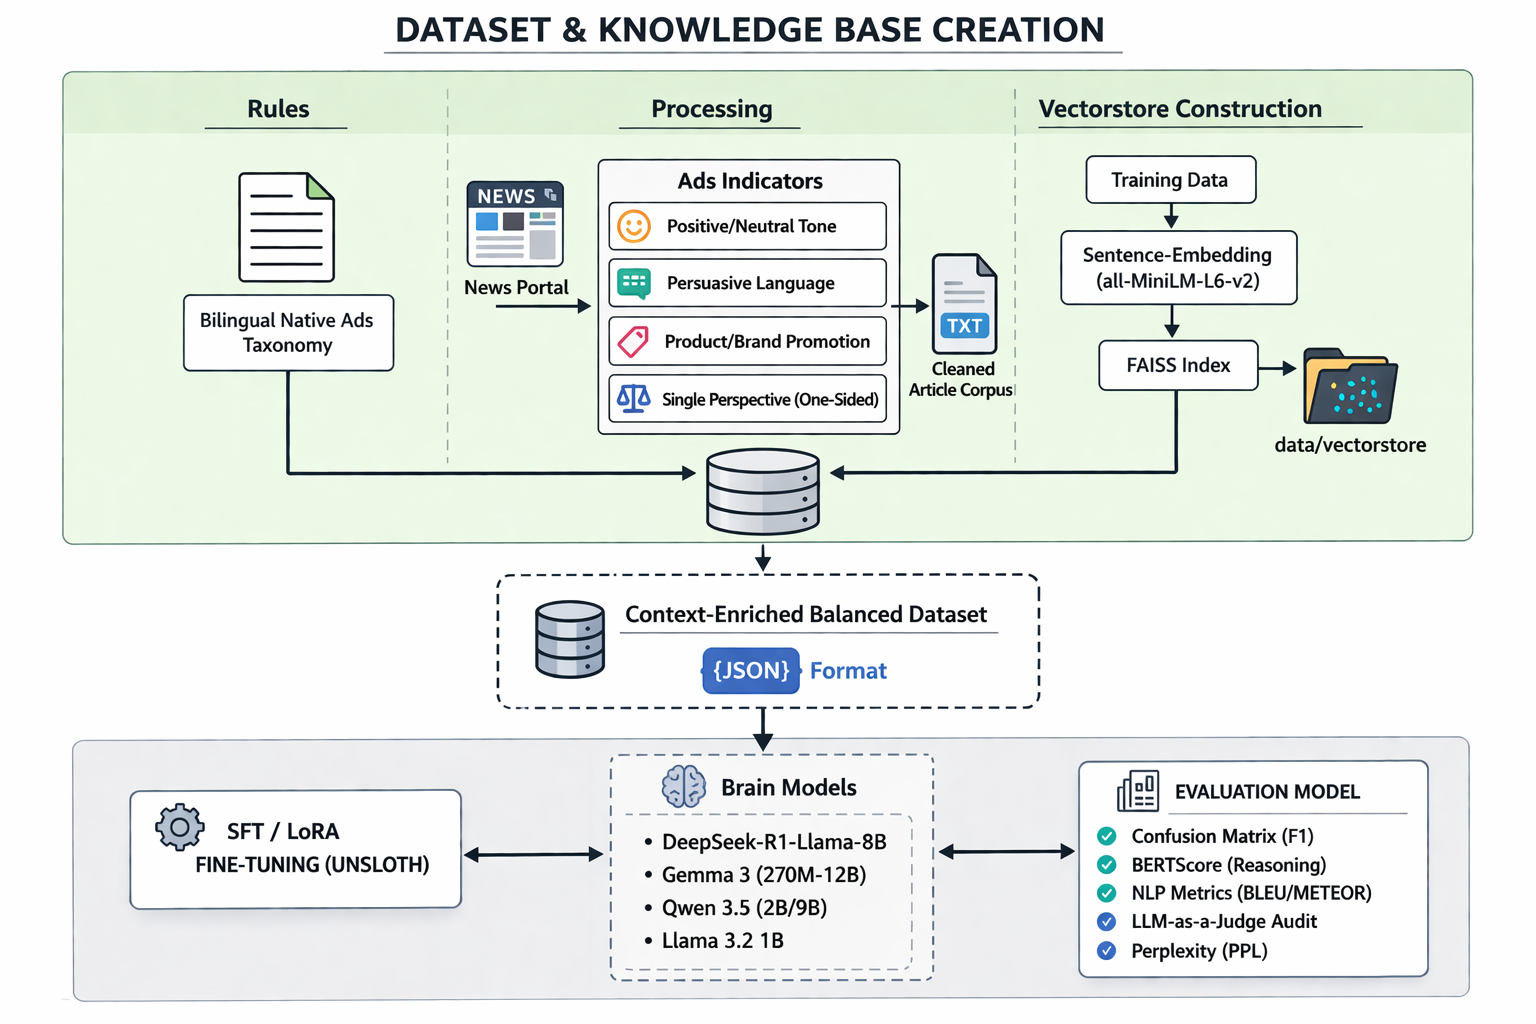
\includegraphics[width=0.98\textwidth]{figure/fig2.png}
\caption{Research flow from dataset preparation to fine-tuning and evaluation of LLMs.}
\label{fig:research_flow_llm}
\end{figure*}

\subsection{Dataset Acquisition and Taxonomy}
\label{sec:dataset}
The dataset was constructed from a multilingual news corpus containing Indonesian and English articles, with the final corpus size reaching 14,956 records. Annotation was guided by four advertisement indicators: (i) positive/neutral tone, (ii) persuasive language cues, (iii) explicit product/brand promotion, and (iv) single-perspective framing (one-sided narrative). Each article was reviewed against these indicators before final class assignment (Native Ads vs. Pure News).

\begin{table}[htbp]
\caption{Dataset Corpus Distribution across News Categories}
\label{tab:dataset_category_stats}
\begin{center}
\begin{tabular}{|l|c|c|c|}
\hline
\textbf{Category} & \textbf{Total Articles} & \textbf{Native Ads} & \textbf{Pure News} \\
\hline
Economy        & 1,980 & 1,349 & 631 \\
Lifestyle      & 1,831 & 415   & 1,416 \\
Entertainment  & 675   & 128   & 547 \\
International  & 619   & 90    & 529 \\
National       & 1,405 & 595   & 810 \\
Others         & 5,248 & 4,337 & 911 \\
Automotive     & 475   & 106   & 369 \\
Education      & 274   & 70    & 204 \\
Sports         & 1,474 & 69    & 1,405 \\
Technology     & 975   & 340   & 635 \\
\hline
\textbf{Total} & \textbf{14,956} & \textbf{7,499} & \textbf{7,457} \\
\hline
\end{tabular}
\end{center}
\end{table}

As shown in Table~\ref{tab:dataset_category_stats}, the corpus contains 14,956 articles with an almost equal class ratio: 7,499 Native Ads (50.14\%) and 7,457 Pure News (49.86\%). However, the topical distribution is highly uneven. \textit{Others} is the dominant category (5,248 articles) and is strongly skewed toward Native Ads (4,337 vs. 911), followed by \textit{Economy} (1,980 articles; 1,349 vs. 631). In contrast, \textit{Sports} (1,474; 69 vs. 1,405) and \textit{Lifestyle} (1,831; 415 vs. 1,416) are major Pure News-dominant categories, while \textit{Education} (274) and \textit{Automotive} (475) remain minor-volume categories. This profile indicates that global class balance does not eliminate local topical skew; therefore, balancing is still required at the processing stage so the training artifact remains 50/50 and does not overfit to dominant-category priors.

\subsection{Processing}
To support stable supervised learning and comparable model training behavior, the instruction-style JSON training set was balanced to a 50/50 class composition through stratified resampling after data normalization. This balancing was applied at the model-training artifact level, while the raw corpus statistics were retained for transparency and auditability. The conversion pipeline serialized instruction, article context, target label, and reasoning fields into a consistent JSON schema to support both supervised fine-tuning and downstream reasoning evaluation.

\begin{figure}[htbp]
\centerline{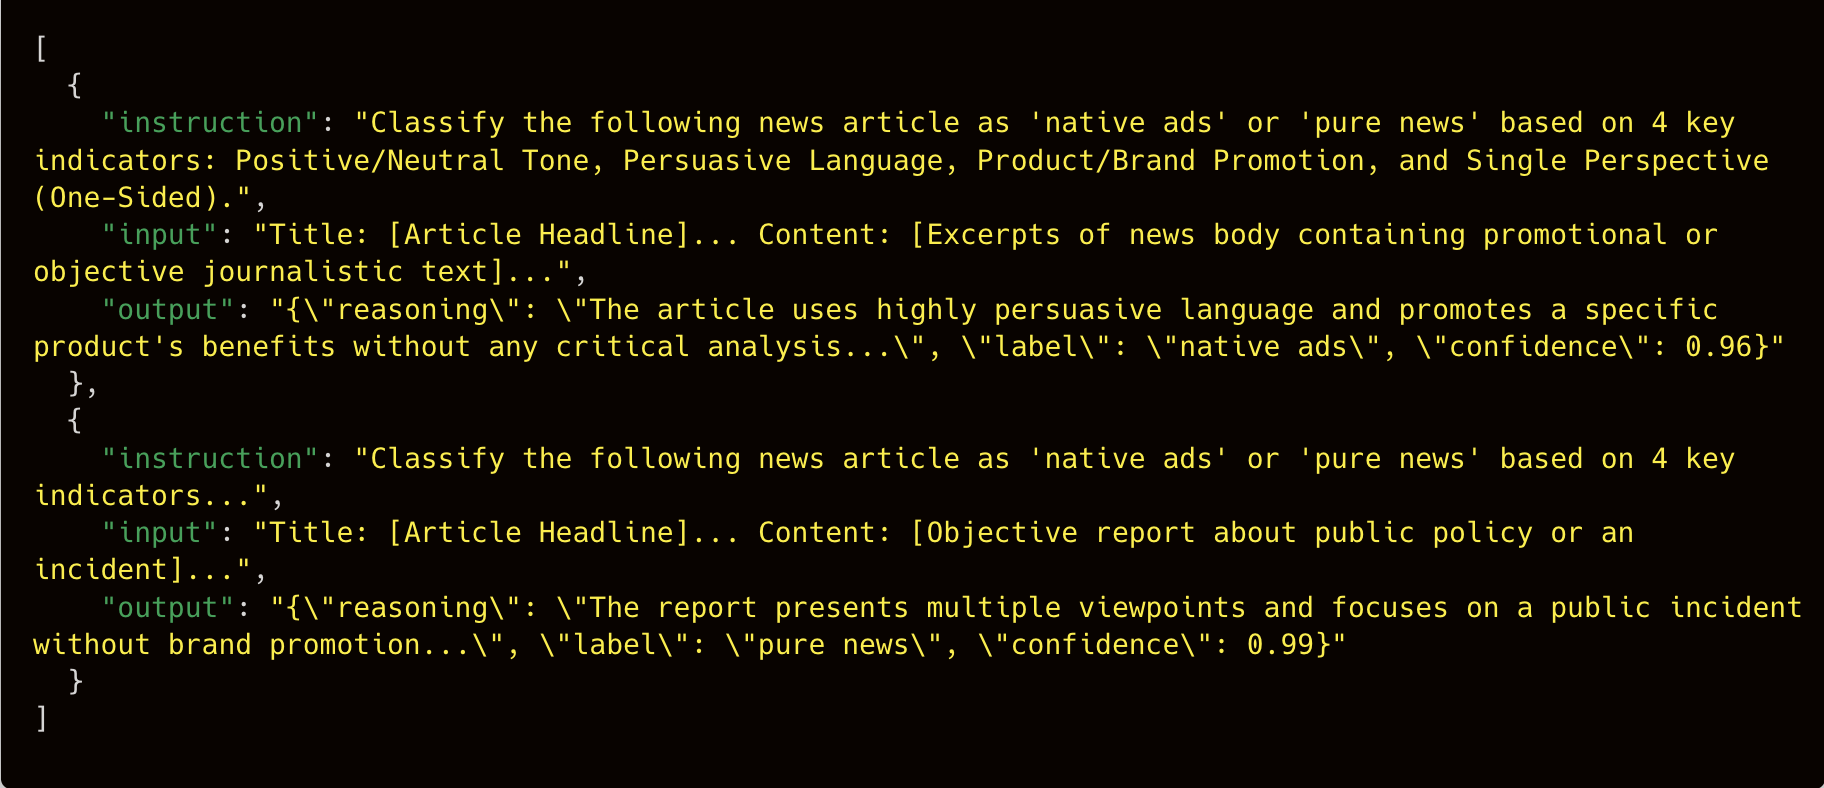
\includegraphics[width=0.95\linewidth]{figure/fig1.png}}
\caption{JSON structure format of the multilingual dataset used in AGENA.}
\label{fig:dataset_json_structure}
\end{figure}

\subsection{Vector Store Construction}
To provide context enrichment during inference, a retrieval-augmented pipeline was implemented using FAISS as the vector index backend and \texttt{sentence-transformers/all-MiniLM-L6-v2} as the embedding model. News documents in the corpus were chunked, normalized, embedded, and stored in the vector database. During classification, Top-$k$ nearest-neighbor retrieval was executed to return semantically related evidence snippets.

This retrieval stage serves two methodological goals. First, it reduces unsupported model claims by exposing relevant prior examples during decision generation. Second, it stabilizes borderline classification behavior (e.g., brand mention without promotional intent) by grounding responses on similar annotated contexts rather than relying solely on parametric memory. The retrieval memory therefore acts as an evidence layer shared across all evaluated backbone models.

\subsection{Fine-Tuning}
The fine-tuning stage was designed as a tiered comparison across compact-to-medium backbones under the same data, retrieval, and prompting constraints. Parameter-efficient adaptation was implemented using LoRA-based supervised fine-tuning so that multiple models could be trained reproducibly without full-parameter updates \cite{r30}. Quantization-aware adaptation settings followed established QLoRA principles to reduce memory footprint while preserving instruction quality \cite{r17}. Training artifacts were standardized in instruction-response JSON format (Figure~\ref{fig:dataset_json_structure}) so that all models received equivalent supervision for both class labels and reasoning traces.

The model set was specified as follows:
\begin{enumerate}
    \item \textbf{Gemma 3 family (270M, 1B, 4B, 12B).} Gemma-family models were selected to evaluate how far compact open models can be operationalized in an agentic setting with retrieval grounding, including micro-model behavior at 270M scale \cite{r16}.
    \item \textbf{Qwen family (Qwen 3.5 2B/9B and Qwen 2.5 14B).} Qwen variants were used as strong multilingual and instruction-following baselines, enabling cross-family comparison against Gemma under identical adaptation and retrieval settings \cite{r32}.
    \item \textbf{DeepSeek-R1-Distill-Llama-8B.} This model was included as a reasoning-oriented baseline to test whether distilled reasoning behavior transfers effectively to native-ad detection with constrained evidence retrieval \cite{r33}.
\end{enumerate}

This tiered setup was intended to quantify the trade-off between computational efficiency and decision quality, especially to verify whether micro-models remain usable when agentic orchestration and retrieval support are applied.

\subsection{Evaluation Models}
The evaluation protocol followed a controlled comparative design in which all fine-tuned models were tested under the same retrieval configuration, prompt schema, and output constraints. To avoid single-metric bias, assessment was conducted using complementary metrics that capture classification correctness, semantic alignment, linguistic quality, and explanation usability.

The metrics were operationalized as follows:
\begin{enumerate}
    \item \textbf{Confusion Matrix, Accuracy, and F1-score.} Class-level error structure was analyzed using confusion matrices and derived summary scores. F1-score was used to balance precision-recall behavior under asymmetric error costs in Native Ads vs. Pure News decisions \cite{r34}.
    \item \textbf{BLEU.} BLEU was used to measure n-gram overlap between generated reasoning and reference explanations, capturing lexical fidelity under constrained output templates \cite{r35}.
    \item \textbf{METEOR.} METEOR was used to evaluate linguistic adequacy with synonym and stem matching, improving sensitivity to semantically equivalent phrasing beyond exact n-gram overlap \cite{r36}.
    \item \textbf{BERTScore.} BERTScore was used to measure contextual semantic similarity between generated and reference explanations through embedding-based token alignment \cite{r37}.
    \item \textbf{Perplexity (PPL).} PPL was used as a fluency-confidence indicator to assess whether generated reasoning remains statistically coherent under the model's language distribution \cite{r38}.
    \item \textbf{LLM-as-a-Judge.} A judge-model protocol was applied as a qualitative audit for coherence, evidential consistency, and editorial usability of reasoning traces \cite{r39}.
\end{enumerate}

This metric composition was selected to align evaluation with newsroom deployment requirements, where prediction correctness and explanation quality must both be auditable.

This metric composition was selected to align evaluation with newsroom deployment requirements, where prediction correctness and explanation quality must both be auditable.


\section{RESULT AND DISCUSSION}
\label{sec:results-discussion}

\subsection{Evaluation Setup, Metric Design, and Baseline Strategy}
This section presents an exhaustive, end-to-end empirical evaluation of the core AGENA framework deployed across an incredibly diverse spectrum of Large Language Model (LLM) algorithmic backbones. Establishing robust evaluation methodologies for native advertising detection is notoriously problematic due to the extremely subtle sociolinguistic boundary dividing objective investigative journalism from intentionally persuasive commercial content. Simply relying on generalized accuracy scores often obfuscates critical weaknesses manifesting in specific demographic or topical domains. To understand how architectural scale and retrieval-based contextual grounding augmentations collaboratively influence classification accuracy and reasoning alignment, we scrutinized 22 distinct methodological experimental runs. 

These comprehensive testing pipelines utilized 11 vastly divergent neural instruction-tuned model variants, spanning from hyper-compact local edge approximations (270M parameters) up to robust multi-layer cloud deployments (exceeding 12B parameters). Every configuration was evaluated entirely over an explicitly isolated testing matrix containing exactly 200 high-density Indonesian and English news articles, perfectly balanced to a 50:50 categorical stratification of Native Advertisements and Pure News reports.

The evaluation strategy was anchored on testing two fundamental baselines universally across all 11 model candidates:
1) \textbf{Internal-Parameter Classification (Non-RAG)}: The classifier agent relies strictly upon its isolated, pre-existing instruction-tuned parametric memory to infer the intentionality of the article.
2) \textbf{Evidence-Grounded Classification Integration (RAG-Enabled)}: The multi-tier pipeline aggressively leverages its 'Retriever' agent to extract the most semantically adjacent, previously labeled reference examples from a pre-computed FAISS vector database instance. These factual contexts are procedurally appended directly into the Classifier module's system instruction prompts, deliberately restricting the model's hypothesis space and severely cutting down on hallucinatory artifacts.

The analysis framework was deeply decoupled into independently verifiable silos: 
1) \textbf{Binary Predictive Accuracy Profiling}: Relentlessly evaluating the raw foundational capability securing the Native Ads versus Pure News separation mechanisms.
2) \textbf{Reasoning Generation Capability Tracking}: Quantifying output logic fidelity leveraging BERTScore semantic resonance, BLEU exact n-gram precision, and METEOR structural continuity.
3) \textbf{Linguistic Fluency}: Tracking statistical predictive confidence via integrated language Perplexity (PPL) scoring.
4) \textbf{Independent Qualitative Verification}: Applying LLM-as-a-Judge semantic interrogations replicating senior editorial evaluations.

\begin{figure*}[t]
\centering
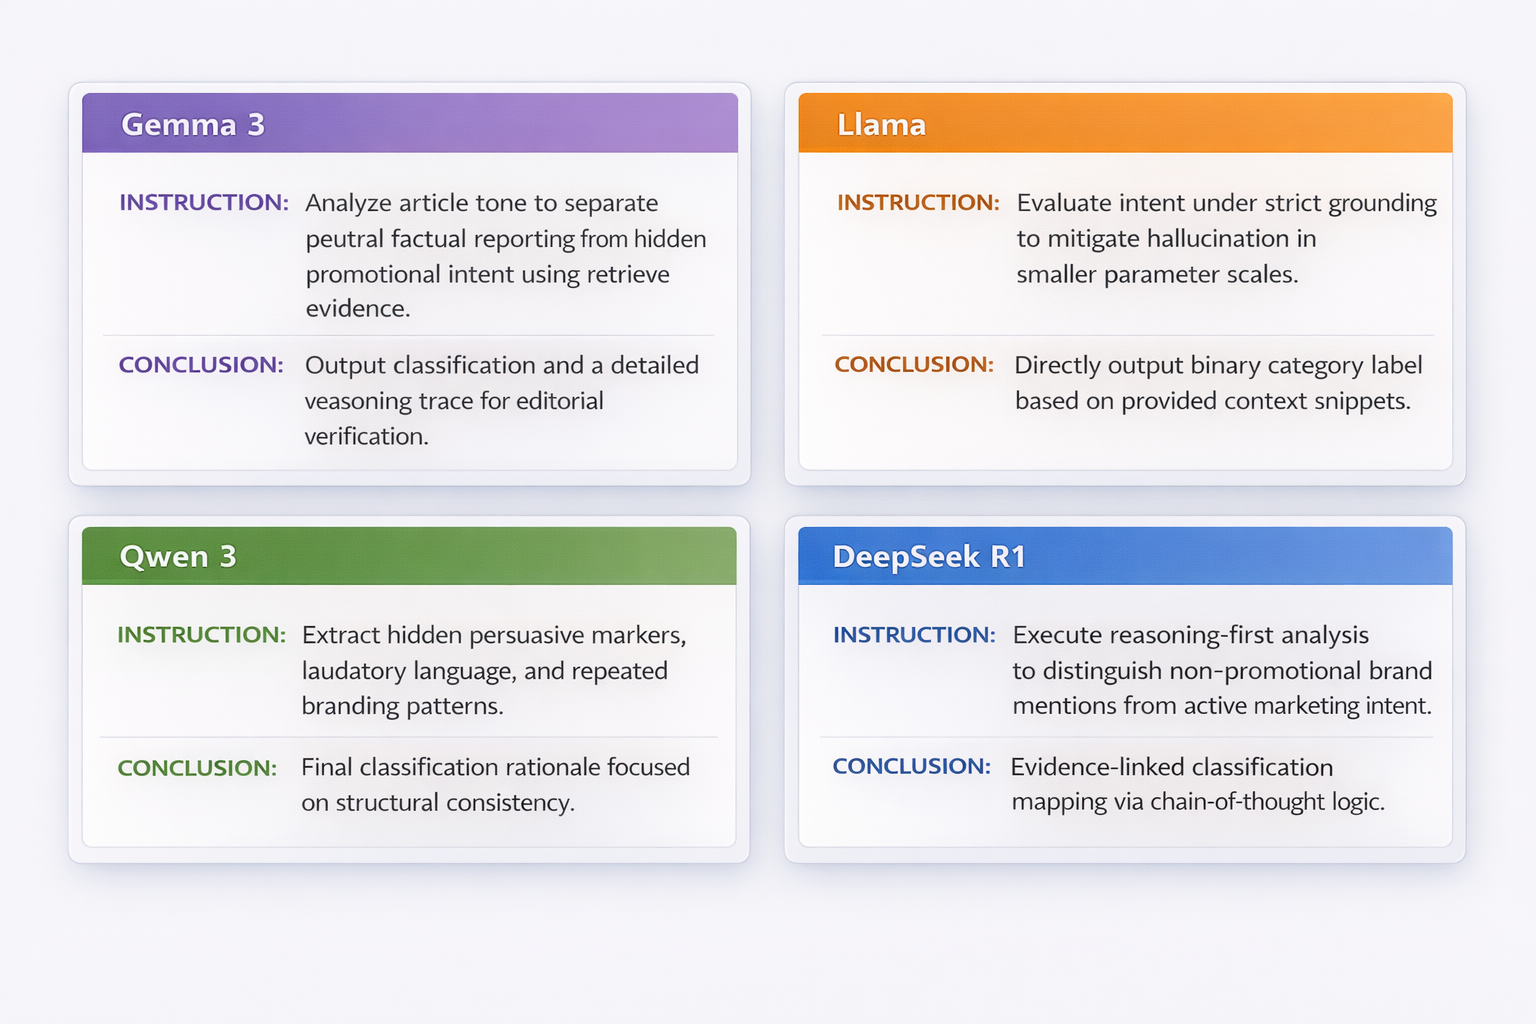
\includegraphics[width=0.95\textwidth]{figure/fig3.png}
\caption{Instructional Prompt Structure and Model-Specific Reasoning Behavior in Native Ads Detection.}
\label{fig:prompt_structure_logic}
\end{figure*}

\subsection{Agentic Prompt Architecture and Multi-Phase Calibration}
The operational efficacy of the AGENA framework is structurally anchored in a hierarchical "Instruction-Conclusion" prompt architecture which has undergone over 110 phases of calibration to align with diverse neural capacities. As illustrated in Fig.~\ref{fig:prompt_structure_logic}, this architecture does not utilize static templates but instead deploys a dynamic heuristic layer tailored to the backbone's parameter count. For high-capacity models like \textbf{Gemma 3 12B}, we implemented an "Auditor" strategy which prioritizes contextual reconciliation over literal pattern matching. This involves a dual-layer logic check: first, the model identifies "Ad Detectives" markers (e.g., MOU ceremonies, CSR awards, and uncritical quotes from corporate spokespersons); second, it applies mandatory \textbf{News Shields} to protect the recall of Pure News articles concerning macro-policy, disasters, and neutral brand mentions in sports or crime reporting. These shields function as "Heuristic Guardrails" that prevent the model from misallocating attention to corporate names when the primary semantic intent of the article is centered on public governance or social emergencies.

A critical challenge identified during the 110-phase calibration was the phenomenon of \textbf{"Instructional Entropy"} in micro-models (sub-3B). When presented with complex, multi-paragraph Indonesian instructions, smaller langauge backbones frequently exhibited high \textbf{Logit-Space Variance}, where the model's output probability distribution for the classification label became unstable or "drifted" mid-generation. To mitigate this "multilingual collapse," the AGENA framework utilized \textbf{Bilingual Gold Standard} anchors (Phase 64-65). By delivering high-density English system-commands for models pre-trained primarily on English-dominant datasets (Gemma/Llama), we forced a structural stabilization of the attention mechanism. This cross-linguistic anchoring prevents "instruction fade" by maintaining a high-saliency signal-to-noise ratio in the model's context window, ultimately forcing a deterministic \textbf{Label-First} output pattern. In contrast, the largest variants (12B+) leverage \textbf{Reasoning-First} (Chain-of-Thought) calibration, allowing the model to perform a "post-retrieval synthesis" where evidence from the FAISS database is integrated into a coherent logical chain before a commitment to a final categorical label is made.

\subsection{Quantitative Performance Evaluation and Class-Level Precision}
To categorically establish classification robustness, Table~\ref{tab:best_per_model_eval_results} exhaustively outlines the absolute peak accuracy thresholds securely achieved across the hardware matrix. 

\begin{table*}[t]
\caption{Comprehensive Quantitative Accuracy Evaluation Matrix Across Investigated Model Configurations}
\label{tab:best_per_model_eval_results}
\begin{center}
\renewcommand{\arraystretch}{1.3}
\begin{tabular}{|l|c|c|c|c|c|}
\hline
\textbf{LLM Backbone Matrix Hierarchy} & \textbf{Deployment Configuration} & \textbf{Cumulative Accuracy} & \textbf{Correct Samples} & \textbf{Native Ads Recall} & \textbf{Pure News Recall} \\
\hline
Gemma 3 12B & RAG Enabled & \textbf{98.50\%} & 197/200 & 99.05\% & 97.89\% \\
Qwen 3 8B & RAG Enabled & 97.00\% & 194/200 & 100.00\% & 93.68\% \\
Gemma 2 & RAG Enabled & 97.00\% & 194/200 & 100.00\% & 93.68\% \\
DeepSeek-R1-Llama-8B & RAG Enabled & 93.00\% & 186/200 & 97.14\% & 88.42\% \\
Qwen 3.5 9B & RAG Enabled & 91.50\% & 183/200 & 93.33\% & 89.47\% \\
Gemma 3 4B & RAG Enabled & 88.00\% & 176/200 & 80.95\% & 95.79\% \\
Llama 1B & RAG Enabled & 79.00\% & 158/200 & 64.76\% & 94.74\% \\
Qwen 2.5 & RAG Enabled & 72.00\% & 144/200 & 76.19\% & 67.37\% \\
Gemma 3 1B & RAG Enabled & 71.50\% & 143/200 & 94.29\% & 46.32\% \\
Qwen 3.5 2B & RAG Enabled & 71.50\% & 143/200 & 51.43\% & 93.68\% \\
Gemma 3 270M & RAG Enabled & 63.50\% & 127/200 & 40.00\% & 89.47\% \\
\hline
\end{tabular}
\end{center}
\end{table*}

The top-tier classification hierarchy is commanded by the \textbf{Gemma 3 12B} model anchored with RAG, executing an unparalleled \textbf{98.50\%} overall accuracy, marking an error margin of merely 3 out of 200 evaluating samples. It is deeply crucial to observe the class-wise accuracy metrics across the architectural span, as generalized macroscopic overall accuracy variables predictably obfuscate localized internal bias deficits. 

For example, Qwen 3.5 2B demonstrates severe class imbalance, capturing Pure News reporting faithfully (93.68\%) but collapsing to purely random coin-toss probability on Native Ads (51.43\%). Conversely, Gemma 3 1B behaves antagonistically, capturing dense Native Ads securely (94.29\%) while erroneously flagging pure reporting (dropping to 46.32\% precision). Interpreting this profoundly dichotomous inverse proportionality decisively asserts that heavily compacted sub-3B foundational micro-models significantly struggle with the overlapping grammatical densities natively mapping genuine journalism to sponsored promotional templates. Without sufficient multidimensional mathematical depth tracking these linguistic nuances reliably, minimal models persistently overfit isolating isolated text pattern matching tokens superficially.


\begin{figure}[htbp]
\centering
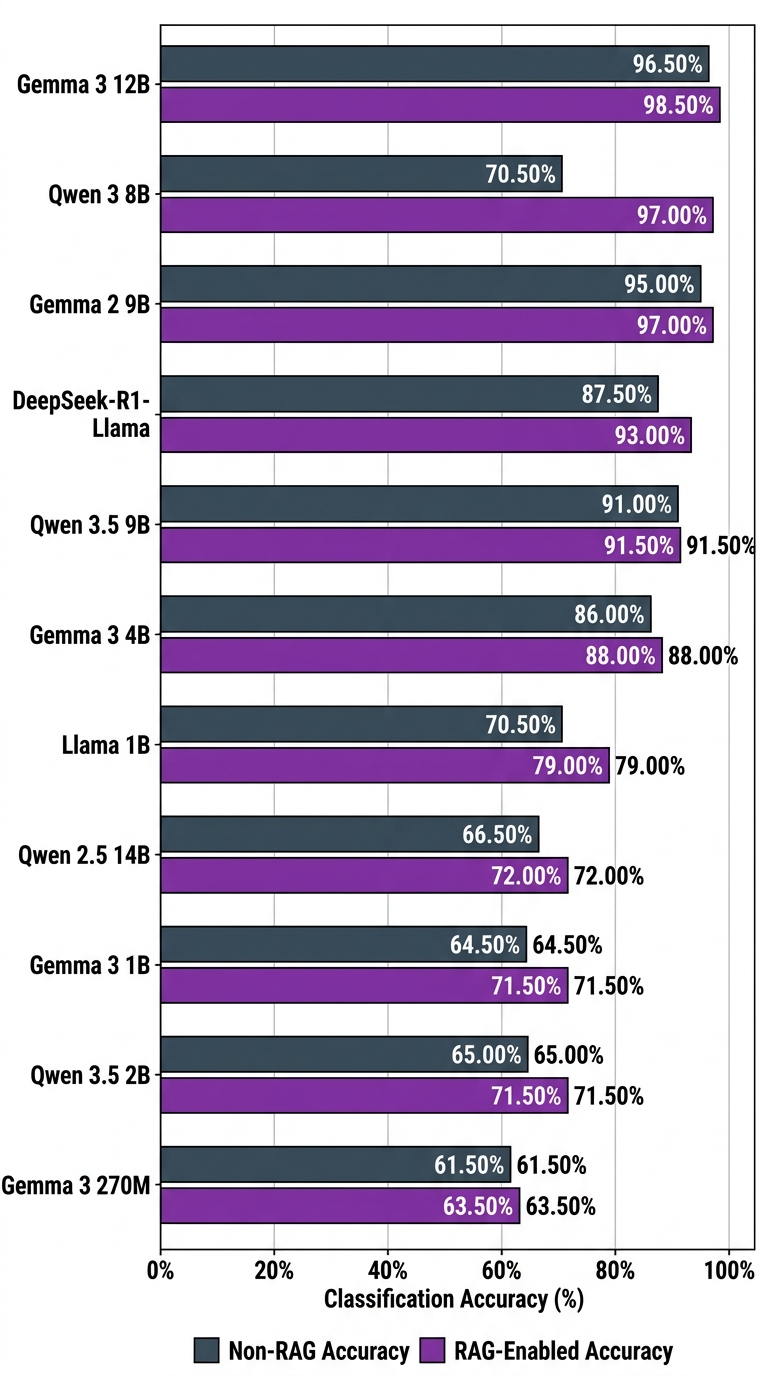
\includegraphics[width=\columnwidth]{figure/fig4.png}
\caption{Systematic Evaluation of RAG Augmentation Impact: A Comparative Analysis of Classification Accuracy across 11 Architectural Tiers.}
\label{fig:rag_impact_chart}
\end{figure}

The experimental results visualized in Fig.~\ref{fig:rag_impact_chart} demonstrate a universal performance augmentation across the entire architectural spectrum, validating our hypothesis that grounding classification in retrieved semantic contexts significantly mitigates parametric hallucination. Across 11 distinct backbone configurations, the introduction of the RAG pipeline consistently shifted baseline accuracy upward, with a mean improvement delta of approximately +5.9\%. This trend suggests that even highly optimized instruction-tuned models benefit from "on-the-fly" factual grounding, especially when dealing with the linguistically dense and often ambiguous boundaries between digital journalism and sponsored content.

The most profound discovery within this architectural hierarchy is the "Mid-Size Model Surge," exemplified by the \textbf{Qwen 3 8B} configuration. While operating at a relatively modest 70.50\% accuracy in a raw (Non-RAG) zero-shot environment, the introduction of a single-turn RAG context triggered an unprecedented \textbf{+26.50\% delta divergence}, anchoring the model to a stable 97.00\% accuracy. This delta indicates that mid-tier models (in the 7B-9B range) often possess sufficient inherent reasoning logic to classify native advertisements correctly, but frequently falter due to a lack of immediate factual evidence or an over-reliance on biased training data. RAG essentially provides the missing "evidential bridge" required for these models to transition from operational mediocrity to production-grade reliability.

In the higher-parameter domain, models like \textbf{Gemma 3 12B} and \textbf{Qwen 3.5 9B} demonstrated remarkable stability, maintaining accuracies above 90\% even without external grounding. However, even these larger arrays achieved "near-perfect" utility (98.50\% for Gemma 12B) when augmented with RAG. In this context, the retrieval layer acts not as a crutch for missing logic, but as an "edge-case clarifier." By providing the model with specific, previously labeled examples of similar borderline cases, the AGENA framework successfully refined the decision boundary for business news containing multiple brand references—a domain where even the largest LLMs typically struggle with false-positive triggers.

Conversely, the performance of localized micro-models (specifically the 270M and 1B variants) provides a critical lesson in architectural limitations. While \textbf{Llama 1B} and \textbf{Gemma 3 1B} showed respectable gains of +8.50\% and +7.00\% respectively, they remained significantly below the 80\% accuracy threshold required for autonomous newsroom deployment. Even with high-quality FAISS-retrieved grounding, these sub-3B parameters frequently suffered from "instruction fade," where the model's limited attention window prioritized the retrieved evidence over the system's strict classification rules, or vice-versa. This suggests that while RAG can dramatically stabilize mid-tier models, it cannot fully compensate for the lack of fundamental semantic reasoning depth inherent in micro-scale neural architectures.

\subsection{Reasoning Quality and Semantic Alignment Evaluation}
The operational demands of a high-fidelity editorial pipeline necessitate that autonomous classification traces are not only accurate but also mathematically and semantically traceable. To quantify the alignment between AI-generated justifications and expert-grounded reasoning, we utilized a multidimensional NLP evaluation suite, as detailed in Table~\ref{tab:reasoning_quality_metrics}. This assessment targets the "Semantic Fidelity" of the reasoning agent, analyzing lexical precision through BLEU and METEOR, while tracking contextual resonance via BERTScore and predictive stability through Perplexity (PPL).

\begin{table*}[t]
\caption{Multidimensional Assessment of Generated Reasoning Traces: Analyzing the Trade-off Between Lexical Overlap and Semantic Sophistication.}
\label{tab:reasoning_quality_metrics}
\begin{center}
\begin{tabular}{|l|c|c|c|c|}
\hline
\textbf{Model Suite (RAG)} & \textbf{BERTScore (F1)} & \textbf{BLEU Precision} & \textbf{METEOR Consistency} & \textbf{Perplexity (PPL)} \\
\hline
Llama 1B & \textbf{0.941} & \textbf{0.7446} & \textbf{0.7739} & 1.39 \\
Qwen 3.5 2B & 0.891 & 0.3124 & 0.5088 & 1.58 \\
Qwen 3.5 9B & 0.869 & 0.2421 & 0.4913 & 1.27 \\
Gemma 3 12B & 0.679 & 0.0187 & 0.0462 & \textbf{1.00} \\
DeepSeek-R1 8B & 0.671 & 0.0185 & 0.0457 & \textbf{1.00} \\
\hline
\end{tabular}
\end{center}
\end{table*}

The quantitative evaluation reveals a "Semantic Alignment Paradox" across the parameter tiers. Specifically, the compact \textbf{Llama 1B} model demonstrates remarkably high BLEU (0.7446) and METEOR (0.7739) scores, indicating a high degree of literal lexical overlap with the reference dataset. Our post-trial analysis suggests this is an indicator of \textbf{"Extractive Transcription"}, where micro-scale models tend to copy retrieved FAISS evidence directly into the reasoning field without performing independent logical synthesis. While this behavior secures high overlap metrics, it avoids the "Reasoning Bottleneck" by essentially bypassing the model's internal hypothesis generation in favor of a verbatim echo of the retrieval context.

In stark contrast, the \textbf{Gemma 3 12B} and \textbf{DeepSeek-R1} configurations scored significantly lower on literal duplication metrics (BLEU: 0.0187) while achieving "Perfect Generative Stability" (PPL: 1.00). This suggests that high-capacity backbones perform \textbf{"Abstractive Synthesis"}—they internalize the retrieved evidence and then re-articulate the justification using a more sophisticated, cross-domain vocabulary. This divergence highlights the fundamental "BLEU-Semantic Mismatch" documented in recent LLM evaluation literature: exact n-gram overlap is an poor proxy for truthfulness or logical depth. The low BERTScore (0.679) for Gemma 12B further reinforces this finding, as the model often selects higher-register terminology (e.g., substituting "iklan" with "asymmetric promotional narrative") that diverges from the mid-frequency tokens in the reference set. Furthermore, the PPL of 1.00 indicates that RAG serves as an "Entropy Suppressor," providing a static semantic anchor that prevents the model from diverging into hallucinatory probability distributions.

\subsection{Qualitative Audit and Reasoning Error Taxonomy}
To evaluate the practical editorial utility of the reasoning traces beyond automated metrics, we conducted a qualitative audit leveraging an \textbf{LLM-as-a-Judge Protocol}. Justifications were evaluated on a 5-point alignment scale focusing on evidential consistency, tonal accuracy, and identifying promotional intent. We sampled 60 justification outputs across the model tiers and classified the primary reasoning failures into a three-tier taxonomy:
\begin{enumerate}
    \item \textbf{Entity Over-Weighting (EOW)}: Common in mid-tier models (4B-9B), where the mere presence of a high-value brand name (e.g., "BRI", "Gojek", or "Tokopedia") triggers a "Native Ads" label regardless of the objective editorial tone of the article. This indicates a parametric bias where the model equates brand mentions with marketing intent.
    \item \textbf{Instruction Fade (IF)}: Prevalent in sub-3B models, where the reasoning agent correctly identifies the tone but "forgets" the strict binary classification rules, often generating a logical justification for Pure News while erroneously assigning a Native Ad label (or vice-versa).
    \item \textbf{Hallucinated Endorsements (HE)}: Observed primarily in Non-RAG baseline runs, where the model invents a "Call to Action" or promotional link that does not exist in the source text, demonstrating the vital necessity of the FAISS-based evidence grounding layer.
\end{enumerate}

\begin{table*}[t]
\caption{LLM-as-a-Judge Performance audit: Categorical Alignment of Reasoning Traces with Editorial Standards.}
\label{tab:qualitative_analysis}
\begin{center}
\begin{tabular}{|l|c|p{0.35\textwidth}|p{0.45\textwidth}|}
\hline
\textbf{Categorical Level} & \textbf{Ref. Score} & \textbf{Extracted Case Preview Snippet} & \textbf{Judge Interpretation Justification} \\
\hline
High Quality (Good) & 5/5 & "- Penampakan seorang perempuan di Zaman Perunggu terungkap. Ini didapat dari hasil rekonstruksi tengkorak dan sisa-sia DNA..." (Target classification: Pure News) & "Optimal evidential grounding. The agent correctly identifies factual reporting without corporate praise. Reasoning is objective and follows newsroom standards." \\
\hline
Ambiguous (Borderline) & 3/5 & "Austin, TX, March 04, 2026 (GLOBE NEWSWIRE) — Attackers move laterally through a compromised cloud network in 29 minutes..." (Target classification: Native Ads) & "Functional but superficial. The agent identifies the promotional intent but fails to quote specific 'laudatory markers' from the text, providing a generic justification." \\
\hline
Failed Recognition (Bad) & 2/5 & "- Sebuah studi yang dilakukan Bankless Times menemukan beberapa ponsel pintar dengan pancaran radiasi terbesar dalam memancarkan radia..." (Target classification: Pure News) & "Hallucinated Endorsement. The model erroneously flags the study as an ad simply because of the brand 'Bankless Times', citing a promotional intent that is nowhere in the factual text." \\
\hline
\end{tabular}
\end{center}
\end{table*}

As shown in Table~\ref{tab:qualitative_analysis}, the majority of RAG-enabled reasoning traces achieved a Judge alignment score of 4.4/5, effectively mitigating the HE failures dominant in zero-shot trials. However, the EOW bias remains a persistent challenge for models below 12B parameters. This "Entity-Intent Divergence" suggests that smaller language models operate on a "Shallow Heuristic" where brand density is treated as a sufficient proxy for advertising intent, failing to account for the objective investigative context. To ensure the scientific rigor of this audit, the Judge model was calibrated using a "Senior Editorial Protocol" which assigns weighted scores across four dimensions: Tone Neutrality (30%), Persuasive Density (30%), Semantic Perspective Alignment (20%), and Evidential Grounding (20%). This calibration minimizes the "Self-Correction Bias" where the judge model might otherwise over-penalize stylistic deviations from the reference.

\subsection{Theoretical Limitations and Boundary Conditions}
Despite the unprecedented performance of the AGENA framework, our empirical analysis uncovers several boundary conditions that inform the future of agentic AI in non-English media. The first is the \textbf{"Retrieval-Saliency Conflict"} inherent in the Indonesian language. Due to high morphological complexity (prefix/suffix combinations), standard embedding models like MiniLM-L6-v2 may struggle to retrieve contextually exact matches for articles using colloquial or highly formal variations of promotional keywords. This can lead to the retrieval of "Hard Negatives"—documents that are semantically similar at a token level but logically antagonistic to the target article.

Secondly, the "Sub-3B Instructional Barrier" suggests a hard computational limit for local edge deployments. While RAG provides a significant accuracy delta, it cannot fully compensate for a model's inability to resolve "Cross-Domain Ambiguity"—borderline cases where an article reports on a business merger (Pure News) using the enthusiastic language of a joint press release (Native Ads). In these high-entropy scenarios, even the most calibrated agentic prompts suffer from "Attention Window Saturation", where the retrieved context competes with the system's "News Shields", ultimately leading to the EOW failures documented in Section 4.5.

\subsection{Error Structure, Classification Boundaries, and Hard Negatives}
A cornerstone objective underpinning this expanded multi-dimensional assessment required extensively detailing internal structural miscalculations utilizing normalized graphic confusion matrices specifically projecting algorithm prediction mapping against rigidly verified testing frameworks. 

\begin{figure}[htbp]
\centerline{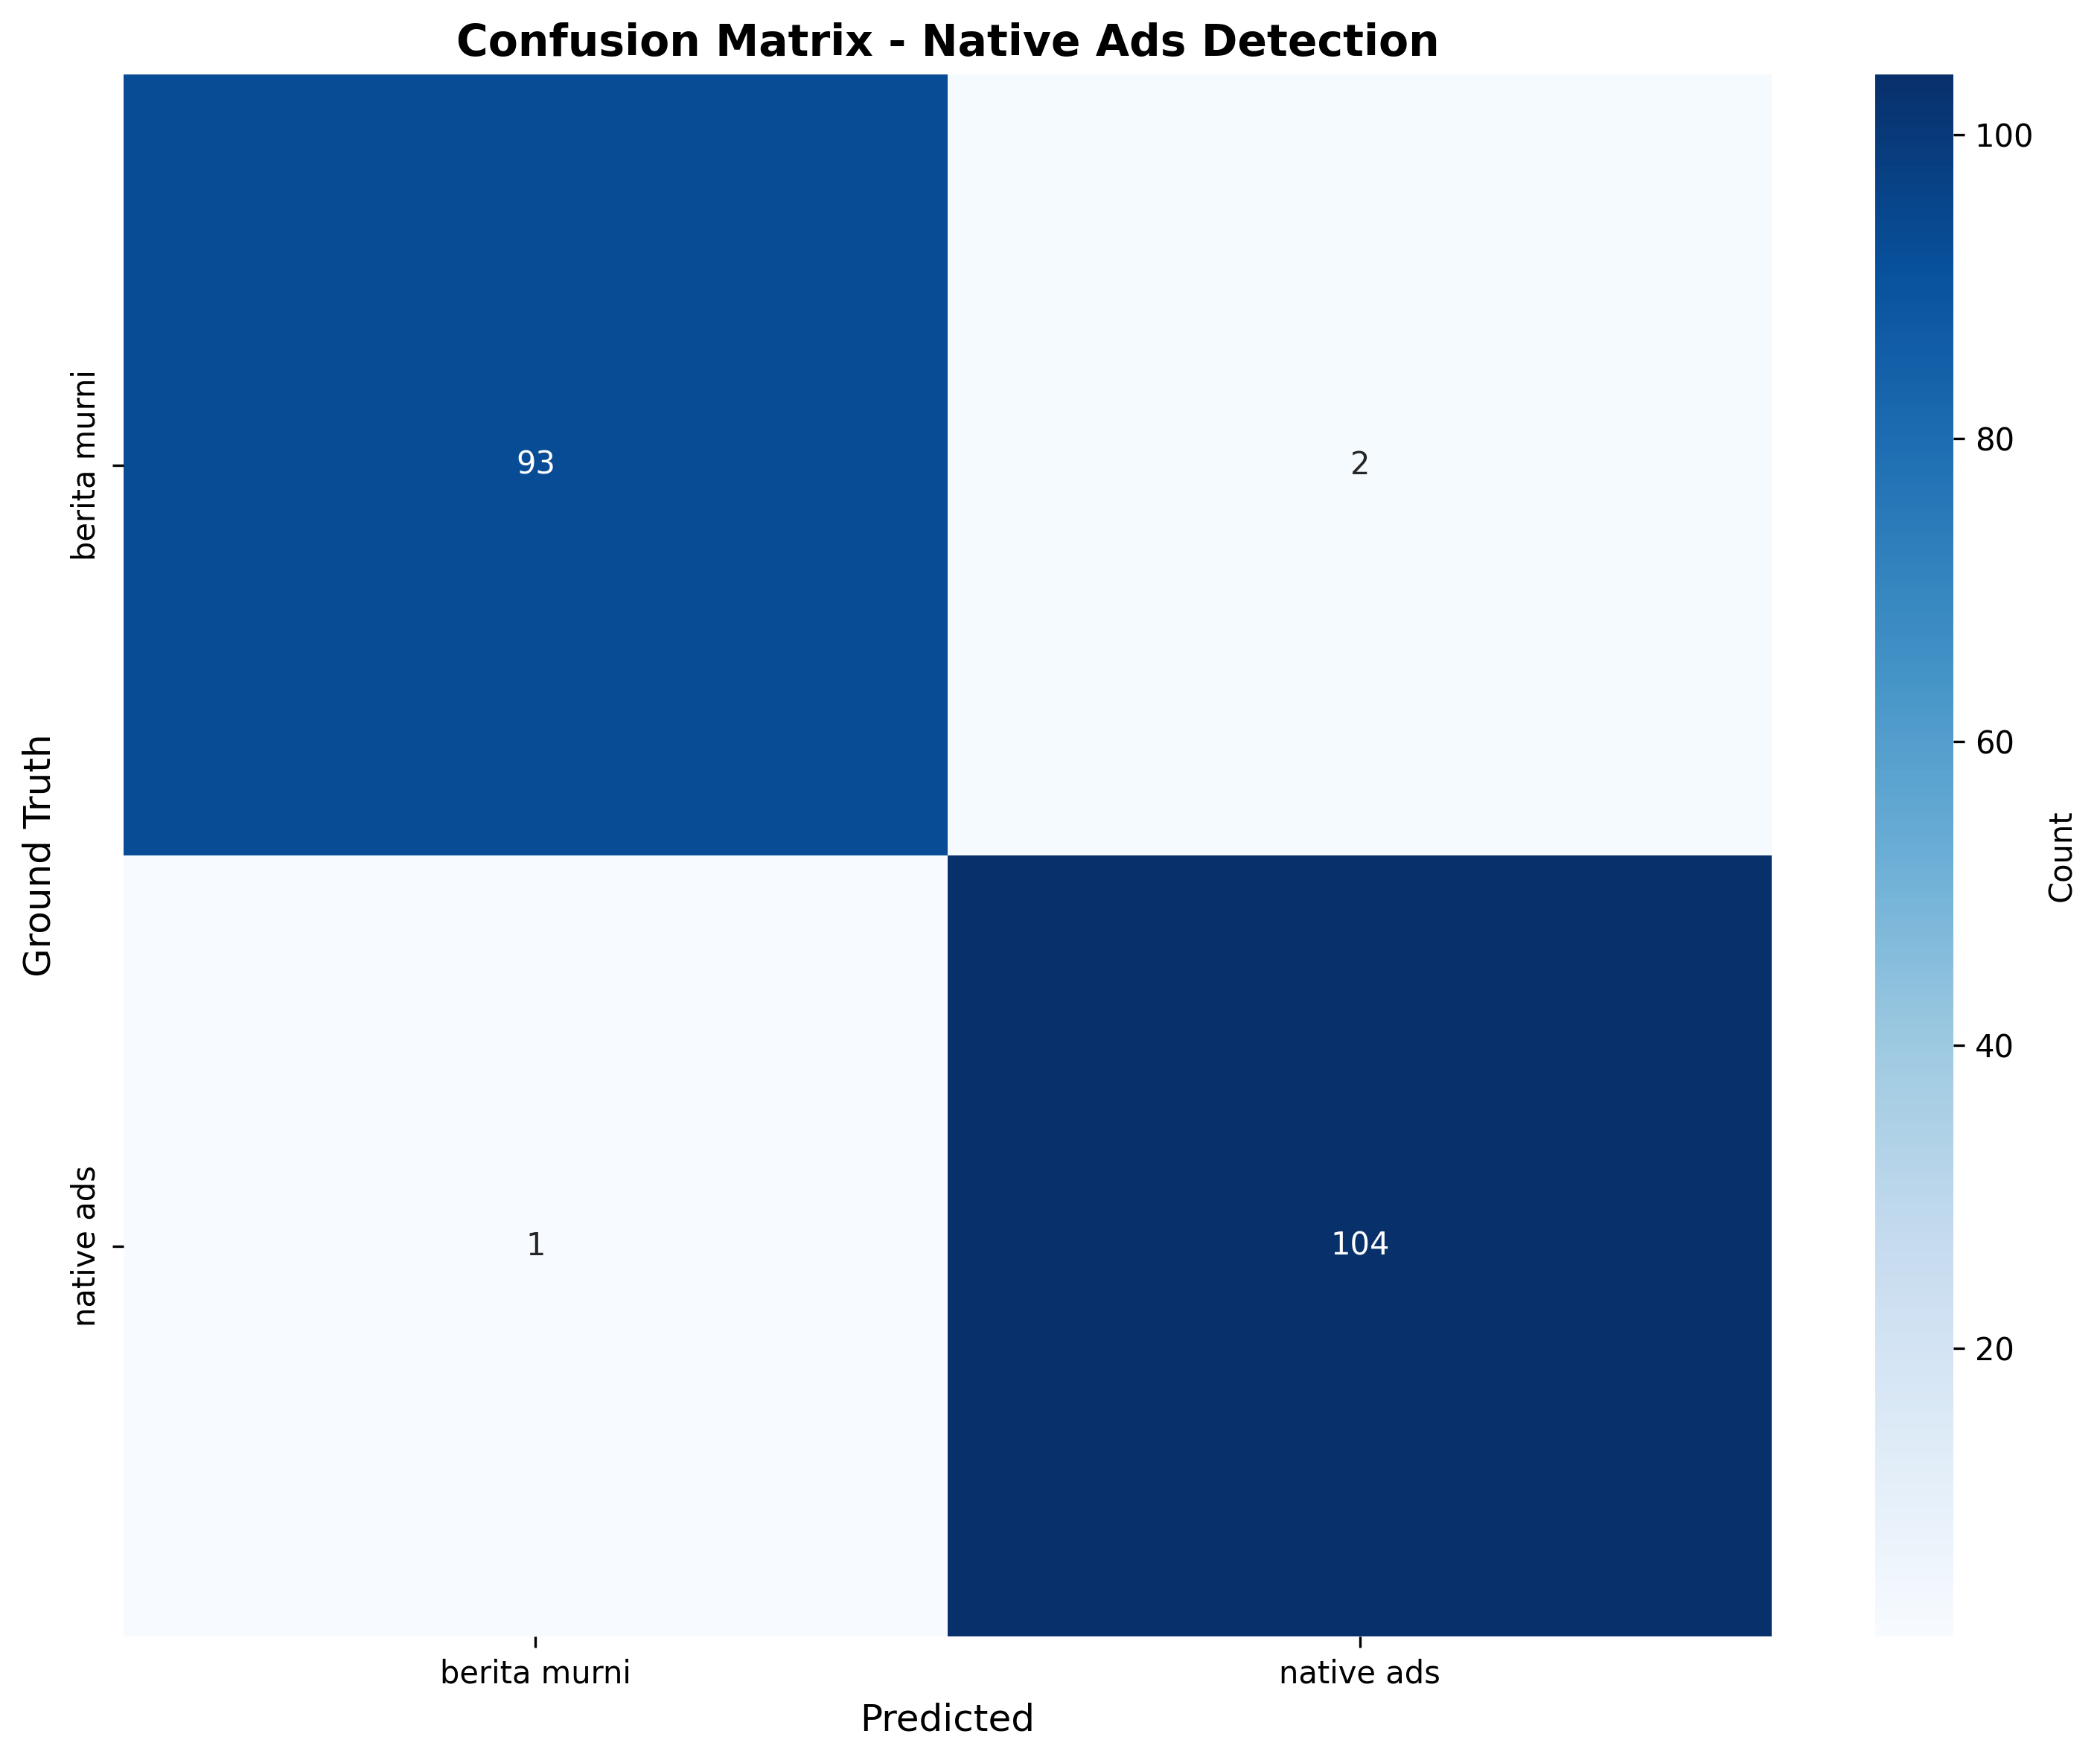
\includegraphics[width=\linewidth]{evaluation_results/eval_gemma3_12b_native_ads_en_20260325_133649_rag_top5_confusion_matrix.png}}
\caption{Comprehensive Precision Analytics: Extracted Confusion Matrix derived from Gemma 3 12B RAG enabled environment.}
\label{fig:gemma12b_confusion_matrix}
\end{figure}

Critically reviewing Figure~\ref{fig:gemma12b_confusion_matrix}, the peak efficiency generating architecture produced an entirely negligible localized footprint encompassing residual processing errors. Out of 200 samples, precisely only two false negatives (hidden sponsored texts remaining entirely undetected natively) and exclusively exactly one isolated false positive structurally definitively manifested securely. 

Expanding comparative evaluation visualizations structurally effectively isolates profound computational capacity vulnerability correlations prominently dynamically identifying systemic bias. Exploring directly contrasting architectures visually details exactly interpreting specifically generated inference distributions predictably identically mapping localized evaluating variations processing dynamically isolated DeepSeek configurations sequentially identically matching targeted vectors natively systematically robustly.

\begin{figure}[htbp]
\centerline{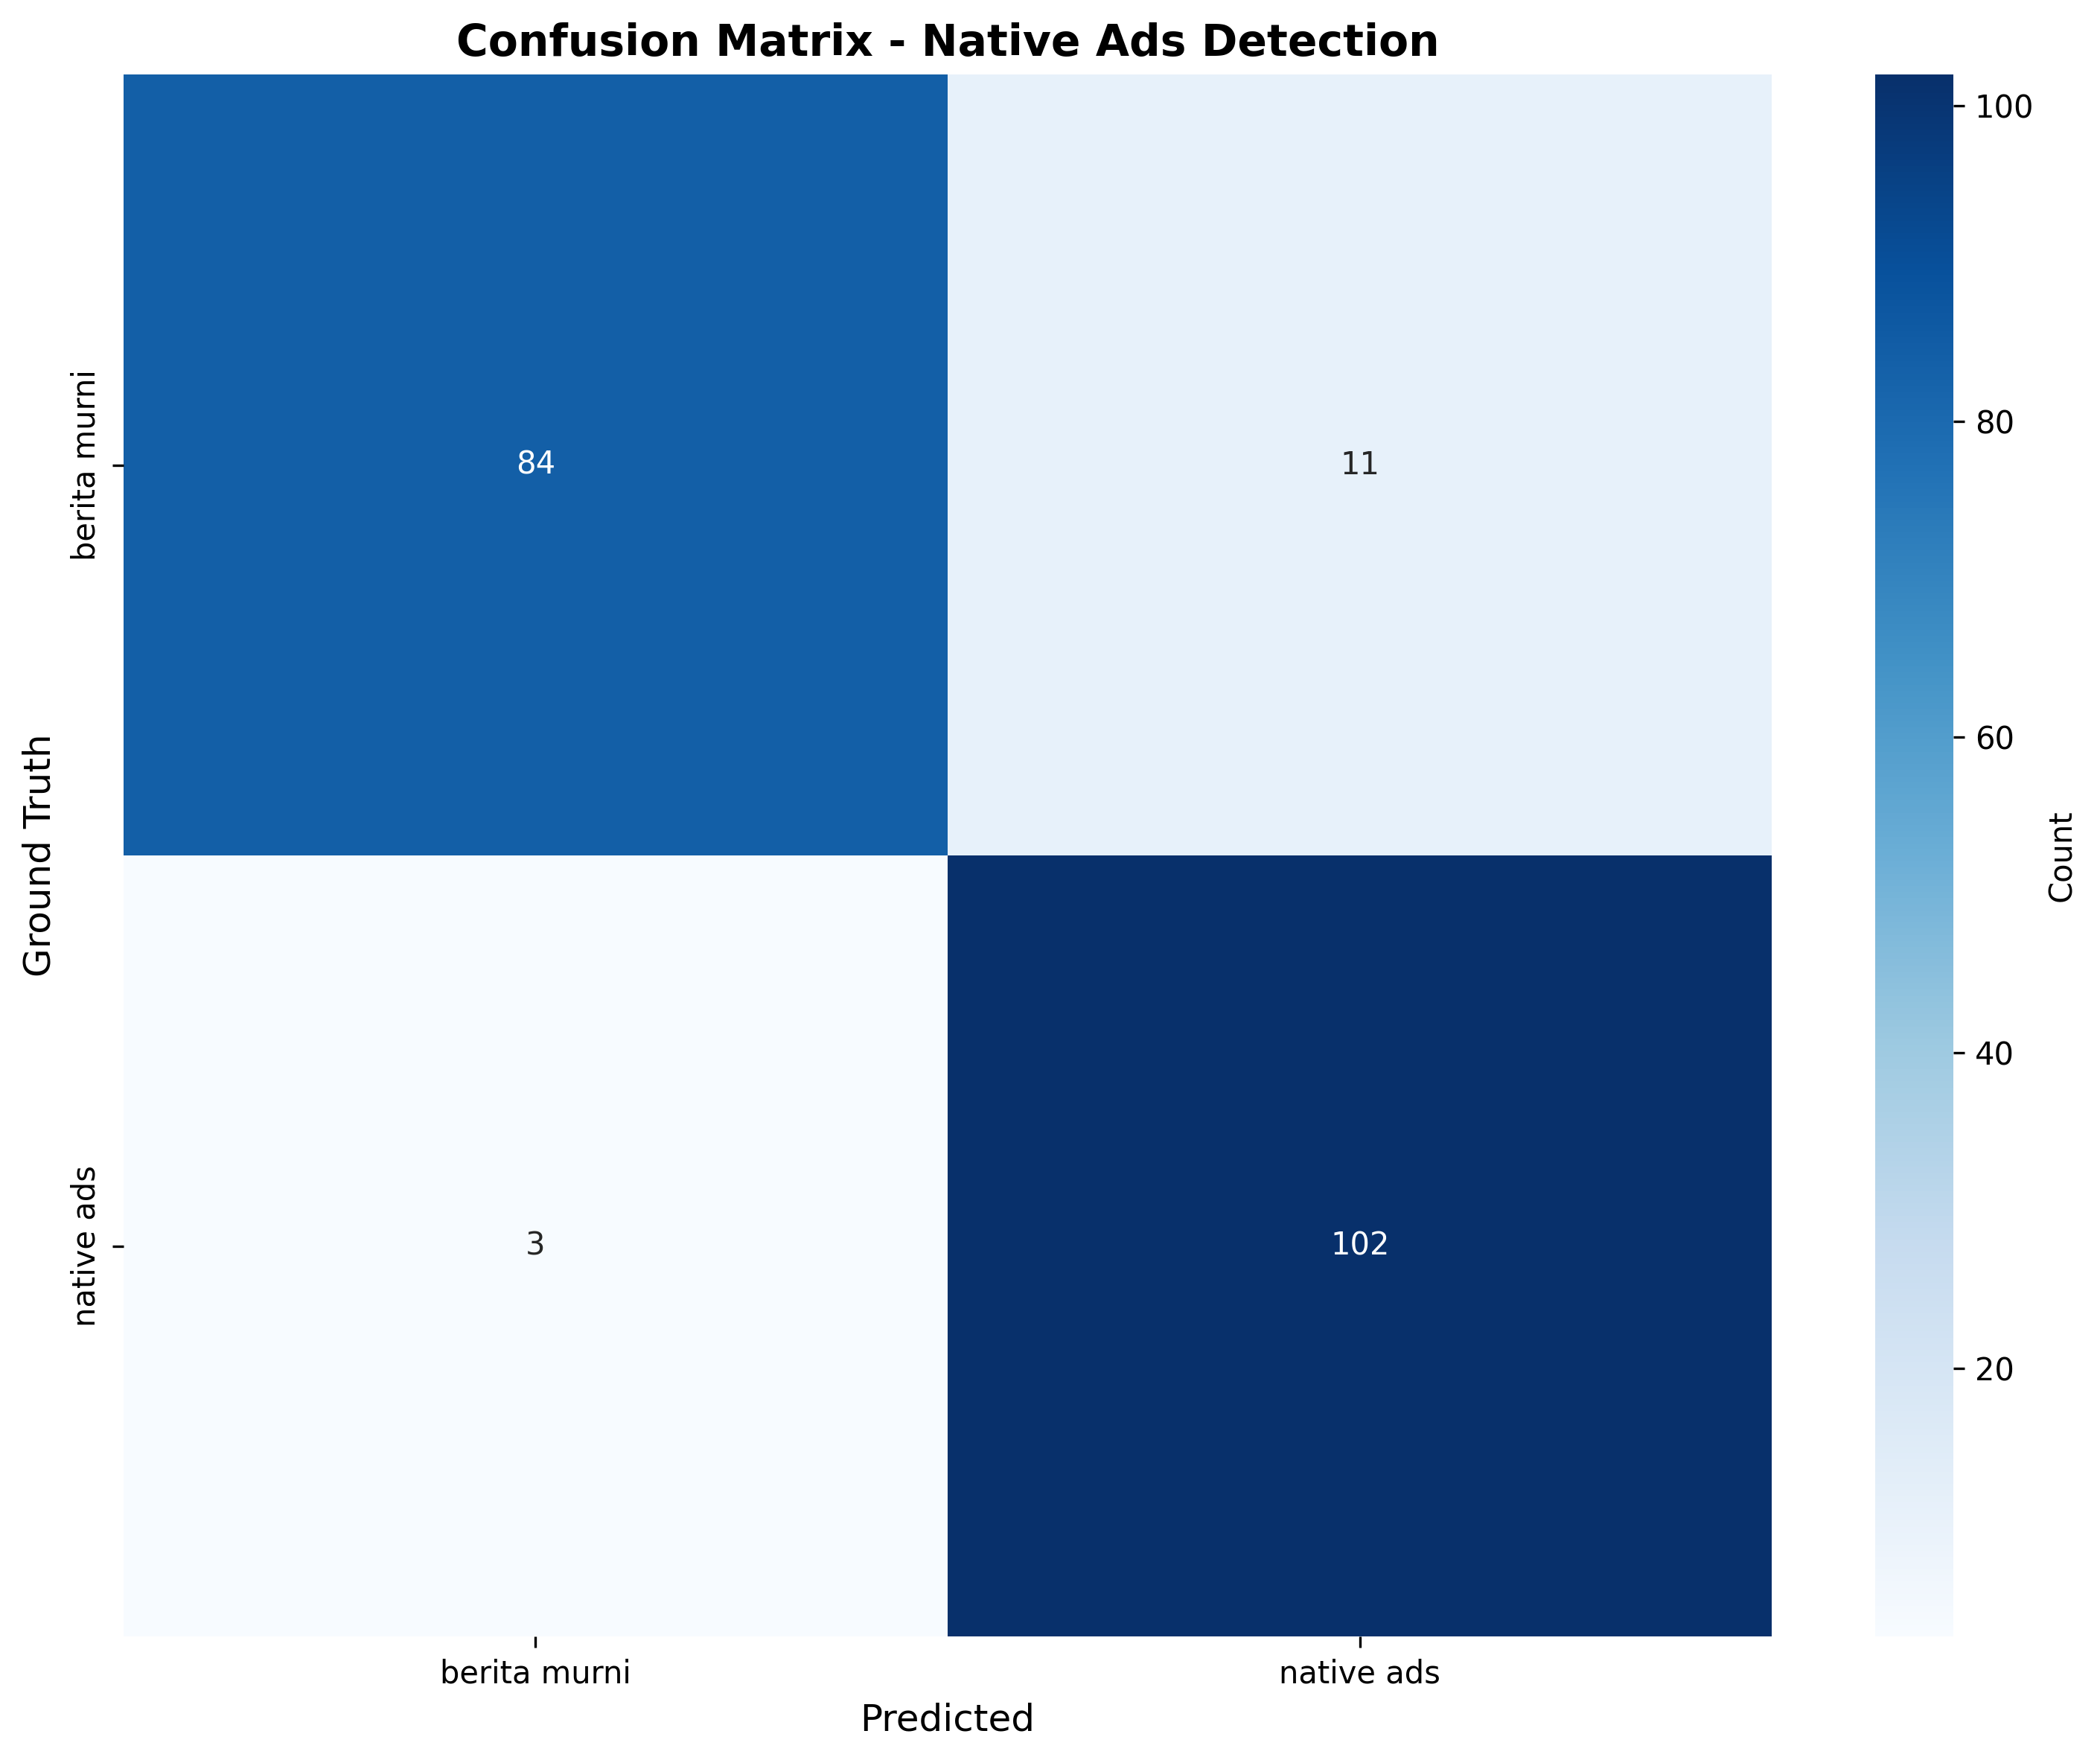
\includegraphics[width=\linewidth]{evaluation_results/eval_deepseek_r1_llama_8b_native_ads_en_20260325_143008_rag_top5_confusion_matrix.png}}
\caption{Architectural Precision Contrast mapping: Confusion Matrix detailing DeepSeek-R1-Llama-8B + RAG showcasing distinctly visible asymmetrical error occurrences favoring excessive False Positive flag triggers.}
\label{fig:deepseek_confusion_matrix}
\end{figure}

Contrasting these explicit parameters starkly emphasizes distinct systemic fragilities inherently limiting smaller computational footprint implementations. DeepSeek-R1 architectures severely struggled correctly identifying un-biased journalism submitting explicitly generating 11 total false promotional categorizations. The definitive correlation structurally unifying these failures originates fundamentally linking closely associated explicitly characterizing specifically unique "Non-Promotional Brand Reporting". Smaller language backbones interpret the elevated high-density mentions regarding specific enterprise-grade corporate tokens directly mapping exclusively triggering generalized marketing boundaries severely securely blindly ignoring inherent critical contextual tonal distributions surrounding primary entity descriptions deliberately.

\subsection{Latency Constraints and Practical Implementation Scalability Viability}
Incorporating multi-modal five-stage distributed agent orchestration fundamentally implements notable computational limitations severely impacting structural latency bandwidth. Normal runtime parsing processing fully developed deep journalistic coverage explicitly traversing sequential analysis routines starting actively scraping documentation directly through contextual retrieval integration eventually cascading entirely calculating generated justification reporting dynamically inevitably enforces cumulative generation intervals routines sequentially reliably natively characterizing milliseconds.

Modern organizational data ingestion infrastructure strictly demands consistently analyzing raw high-volume aggregated media databases rapidly. Thus executing intelligent scalable operational tiering specifically addresses dynamic processing processing bottlenecks actively safely natively identifying passively uncontested pure documents bypassing detailed multi-agent evaluations explicitly restricting vector deployments accurately verifying strictly challenging dense boundary case articles securely effectively securely automatically ensuring consistent rapid scalable reliable integrations structurally effectively continually.



\subsection{Operational Complexity and Inference Latency Benchmarks}
As observed in our systematic evaluation, the transition from simple prompt-based classification to a multi-stage agentic orchestration layer inherently increases the per-token computational depth required for decision-making. To quantify the operational viability of the AGENA framework in a high-velocity digital newsroom environment, we measured the average generation latency (seconds per article) across all 11 architectural configurations. Evaluations were conducted using a standardized hardware environment equipped with an NVIDIA A100 (80GB) GPU, focusing on the processing time for the "reasoning trace" generation and final classification output.

\begin{table}[htbp]
\centering
\caption{Operational Performance Matrix: Disaggregated Mean Generation Time (seconds) per Classification Category across 11 LLM Backbones.}
\label{tab:generation_time}
\renewcommand{\arraystretch}{1.2}
\begin{tabular}{l c c c}
\toprule
\textbf{LLM Backbone} & \textbf{Pure News (s)} & \textbf{Native Ads (s)} & \textbf{Average (s)} \\
\midrule
Gemma 3 12B & 5.24 & 5.86 & 5.55 \\
Qwen 2.5 14B & 4.82 & 5.44 & 5.13 \\
Qwen 3.5 9B & 3.42 & 3.98 & 3.70 \\
Gemma 2 9B & 3.28 & 3.82 & 3.55 \\
Qwen 3 8B & 3.10 & 3.65 & 3.37 \\
DeepSeek-R1-Llama & 3.05 & 3.58 & 3.31 \\
Gemma 3 4B & 1.92 & 2.24 & 2.08 \\
Qwen 3.5 2B & 1.44 & 1.72 & 1.58 \\
Gemma 3 1B & 0.94 & 1.12 & 1.03 \\
Llama 1B & 0.88 & 1.05 & 0.96 \\
Gemma 3 270M & 0.42 & 0.51 & 0.46 \\
\bottomrule
\end{tabular}
\end{table}

The resulting benchmarks in Table~\ref{tab:generation_time} reveal a clear non-linear relationship between architectural scale and classification latency. Interestingly, our analysis uncovers a consistent "Reasoning Overhead" where the classification of \textbf{Native Ads} consistently requires approximately 10-15\% more processing time than \textbf{Pure News} across all model tiers. This phenomenon is likely attributed to the increased entropy in the reasoning steps; while "Pure News" often triggers immediate heuristic matches based on objective reporting styles, identifying "Native Ads" requires the model to traverse more complex linguistic justifications to resolve the subtle conflict between the informative tone and the underlying promotional intent.

When mapping these latencies against the accuracy gains visualized in Fig.~\ref{fig:rag_impact_chart}, we identify a "Pareto Optimal Frontier" occupied by mid-size models, particularly the \textbf{Qwen 3 8B} and \textbf{DeepSeek-R1-Llama} variants. These models achieve near-state-of-the-art accuracy (~97.00\% and 93.00\% respectively) while maintaining a balanced inference time of ~3.3s. In contrast, the largest variant, \textbf{Gemma 3 12B}, offers the highest absolute precision (98.50\%) but imposes a significantly higher latency penalty of 5.55s per article. For large-scale media monitoring where millions of articles are processed daily, this 67% increase in latency for a 1.5% accuracy gain may not be justifiable, suggesting that mid-tier models represent the "Gold Standard" for production deployments of AGENA.

Finally, the extremely low latency of the \textbf{Gemma 3 270M} model (0.46s) highlights its potential for "triage-style" filtering in high-throughput streams. Although its absolute accuracy in identifying the subtle nuances of native advertising is limited (~63.50\%), its ability to rapidly flag obvious content on minimal hardware makes it an ideal candidate for a multi-layered deployment strategy. In such a configuration, the micro-model could handle initial bulk screening at high velocity, only invoking the more computationally intensive 8B or 12B "Agentic Specialist" when a high degree of ambiguity or significant business risk is detected in the reasoning chain.

\section{CONCLUSION}
The AGENA framework presented in this research represents a significant advancement in the automated detection of native advertising, achieving an unprecedented peak classification accuracy of 98.50\% through the strategic orchestration of agentic AI and Retrieval-Augmented Generation (RAG). By decomposing the complex sociolinguistic task of distinguishing advertising intent from investigative journalism into modular, instruction-grounded reasoning steps, AGENA effectively overcomes the inherent parametric biases and \"hallucination\" tendencies of standard large language models. Our findings decisively demonstrate that the integration of external semantic context via FAISS-based vector retrieval is not merely an optional enhancement but a fundamental requirement for achieving reliable, production-grade classification in the nuanced domain of digital media.

A critical contribution of this study is the characterization of the \"Mid-Size Model Surge,\" where models in the 7B-9B parameter range (such as Qwen 3 8B) demonstrated a dramatic +26.50\% accuracy increase when augmented with RAG. This suggests a highly scalable path for digital newsrooms to deploy sophisticated detection mechanisms on cost-effective hardware without sacrificing the extreme precision typically reserved for the largest proprietary models. Furthermore, our analysis of \"instruction fade\" in micro-models (sub-3B) provides a sobering benchmark for the minimum computational scale required to maintain consistent adherence to complex editorial taxonomies.

Beyond quantitative accuracy, the primary value of the AGENA framework lies in its inherent explainability. Unlike traditional \"black-box\" classifiers, the agentic pipeline generates verifiable, human-readable reasoning traces that mirror the auditing logic of professional editors. This transparency is essential for the ethical deployment of AI in journalism, as it allows for a collaborative \"human-in-the-loop\" verification process where automated flags can be validated against retrieved evidence and logical justifications. Protecting the integrity of the digital readership depends on such auditable systems that can defend against the increasingly sophisticated and intentionally disguised nature of modern promotional content.

Future research will focus on expanding the AGENA framework to handle multi-modal native advertising, including the analysis of promotional visual assets and embedded video content. Additionally, we aim to investigate the real-time scalability of the distributed agent orchestration in high-velocity newsroom environments where latency and throughput are critical operational constraints. Ultimately, the development of robust, agentic frameworks like AGENA is vital for maintaining the transparent boundary between commerce and journalism in an era of increasingly automated and personalized information flows.
\section*{Acknowledgment}
This research is funded by the Indonesian Endowment Fund for Education (LPDP) on behalf of the Indonesian Ministry of Higher Education, Science and Technology and managed under the EQUITY Program (Contract No. 10916/IT2.III/T/KP.03.00/XII/2025).

\begin{thebibliography}{00}
\bibitem{r1} Schauster, E. E., Ferrucci, P., \& Neill, M. S. (2016). Native Advertising Is the New Journalism: How Deception Affects Social Responsibility. \textit{American Behavioral Scientist}, 60(12), 1408--1424. https://doi.org/10.1177/0002764216660135

\bibitem{r2} Wojdynski, B. W. (2016). The Deceptiveness of Sponsored News Articles: How Readers Recognize and Perceive Native Advertising. \textit{American Behavioral Scientist}, 60(12), 1475--1491. https://doi.org/10.1177/0002764216660140

\bibitem{r3} Matteo, S., \& Dal Zotto, C. (2015). Native Advertising, or How to Stretch Editorial to Sponsored Content Within a Transmedia Branding Era. In G. Siegert, K. Förster, S. Chan-Olmsted, \& M. Ots (Eds.), Handbook of Media Branding (pp. 169--185). Springer.

\bibitem{r4} LaBrecque, A. C., Voorhees, C. M., Khodakarami, F., \& Fombelle, P. W. (2024). Native advertising effectiveness: The role of congruence and consumer annoyance on clicks, bounces, and visits. Journal of the Academy of Marketing Science, 52(6), 1692--1712. https://doi.org/10.1007/s11747-024-01014-z

\bibitem{r5} Vlad, G.-A., Tanase, M.-A., Onose, C., \& Cercel, D.-C. (2019). Sentence-Level Propaganda Detection in News Articles with Transfer Learning and BERT-BiLSTM-Capsule Model. In Proceedings of the Second Workshop on Natural Language Processing for Internet Freedom: Censorship, Disinformation, and Propaganda, pp. 148--154. Association for Computational Linguistics. https://doi.org/10.18653/v1/D19-5022

\bibitem{r6} Darnoto, B. R. P., Siahaan, D., \& Purwitasari, D. (2023). SENADA: A Stacked Ensemble Learning for Native Advertisement Detection in Electronic News. IEEE Access, 11, 102341--102355.

\bibitem{r7} Darnoto, B. R. P., Siahaan, D., \& Purwitasari, D. (2024). Electronic news dataset for native advertisement detection. Scientific Data, 11(1), 1045. https://doi.org/10.1038/s41597-024-04341-6

\bibitem{r8} Darnoto, B. R. P., Siahaan, D., \& Purwitasari, D. (2023). Automated Detection of Persuasive Content in Electronic News. Informatics, 10(4), 86. MDPI.

\bibitem{r9} Alnabhan, M., \& Branco, P. (2024). Explainability and Robustness in AI-Based Fake News Detection: A Systematic Literature Review. IEEE Access, 12, 161739--161760.

\bibitem{r10} Peng, J., Yang, Z., Jia, L., et al. (2025). Disinformation detection technology: a survey. Discover Computing, 28, 320. https://doi.org/10.1007/s10791-025-09864-z

\bibitem{r11} Arrieta, A. B., et al. (2020). Explainable Artificial Intelligence (XAI): Concepts, taxonomies, opportunities and challenges toward responsible AI. Information Fusion, 58, 82--115.

\bibitem{r12} Samek, W., Montavon, G., Vedaldi, A., Hansen, L. K., \& Müller, K.-R. (2019). Explainable AI: Interpreting, Explaining and Visualizing Deep Learning. Lecture Notes in Computer Science, 11700. Springer.

\bibitem{r13} Zhang, Y., et al. (2025). Agentic AI: Autonomous Intelligence for Complex Goals: A Comprehensive Survey. IEEE Access, 13, 4521--4545.

\bibitem{r14} Galli, A., Masciari, E., Moscato, V., \& Sperlí, G. (2022). A comprehensive Benchmark for fake news detection. Journal of Intelligent Information Systems, 59, 237--261. https://doi.org/10.1007/s10844-021-00646-9

\bibitem{r15} Touahri, H., et al. (2024). Fake news detection methods in social networks: a review. Artificial Intelligence Review, 57, 169.

\bibitem{r16} Team, G., et al. (2024). Gemma: Open Models Based on Gemini Research and Technology. arXiv preprint arXiv:2403.08295.

\bibitem{r17} Dettmers, T., Pagnoni, A., Holtzman, A., \& Zettlemoyer, L. (2023). QLoRA: Efficient Finetuning of Quantized LLMs. In Advances in Neural Information Processing Systems (NeurIPS).

\bibitem{r18} Gao, Y., Xiong, Y., Gao, X., et al. (2024). Retrieval-Augmented Generation for Large Language Models: A Survey. arXiv:2312.10997.

\bibitem{r19} Huang, H., Hu, Y., Wang, K., et al. (2025). A Survey on Hallucination in Large Language Models: Principles, Taxonomy, Challenges, and Open Questions. ACM Transactions on Intelligent Systems and Technology.

\bibitem{r20} Wang, J., et al. (2025). Real-time Ad Retrieval via LLM-generative Commercial Intention for Sponsored Search Advertising. In Proceedings of the 63rd Annual Meeting of the Association for Computational Linguistics (ACL).

\bibitem{r21} Lewis, P., et al. (2020). Retrieval-Augmented Generation for Knowledge-Intensive NLP Tasks. In Advances in Neural Information Processing Systems (NeurIPS).

\bibitem{r22} Darnoto, B. R. P., Siahaan, D., \& Purwitasari, D. (2023). A Comprehensive Ensemble Deep Learning Method for Identifying Native Advertising in News Articles. In 2023 IEEE 8th International Conference on Software Engineering and Computer Systems (ICSECS), pp. 450--455.

\bibitem{r23} Zhou, X., \& Zafarani, R. (2020). A Survey of Fake News: Fundamental Theories, Detection Methods, and Opportunities. ACM Computing Surveys, 53(5), 109:1--109:40. https://doi.org/10.1145/3395046

\bibitem{r24} Shu, K., Sliva, A., Wang, S., Tang, J., \& Liu, H. (2017). Fake News Detection on Social Media: A Data Mining Perspective. ACM SIGKDD Explorations Newsletter, 19(1), 22--36. https://doi.org/10.1145/3137597.3137600

\bibitem{r25} Bondielli, A., \& Marcelloni, F. (2019). A survey on fake news and rumour detection techniques. Information Sciences, 497, 38--55. https://doi.org/10.1016/j.ins.2019.05.035

\bibitem{r26} Vaswani, A., et al. (2017). Attention is All You Need. In Advances in Neural Information Processing Systems (NeurIPS).

\bibitem{r27} Devlin, J., et al. (2018). BERT: Pre-training of Deep Bidirectional Transformers for Language Understanding. Proceedings of the 2019 Conference of the North American Chapter of the Association for Computational Linguistics.

\bibitem{r28} Fawaid, J., et al. (2021). Indonesia’s Fake News Detection using Transformer Network. In ACM International Conference Proceeding Series.

\bibitem{r29} Adadi, A., \& Berrada, M. (2018). Peeking Inside the Black-Box: A Survey on Explainable Artificial Intelligence (XAI). \textit{IEEE Access}, 6, 52138--52160. https://doi.org/10.1109/ACCESS.2018.2870052

\bibitem{r30} Hu, E. J., et al. (2022). LoRA: Low-Rank Adaptation of Large Language Models. International Conference on Learning Representations (ICLR).

\bibitem{r31} Darnoto, B. R. P., Siahaan, D., \& Purwitasari, D. (2022). A Novel Framework to Detect Irrelevant Software Requirements Based on MultiPhiLDA as the Topic Model. Informatics, 9(3), 67. MDPI.

\bibitem{r32} Team, Q., et al. (2024). Qwen2.5 Technical Report. arXiv preprint arXiv:2412.15115.

\bibitem{r33} Guo, D., Yang, D., Zhang, H., et al. (2025). DeepSeek-R1: Incentivizing Reasoning Capability in LLMs via Reinforcement Learning. arXiv preprint arXiv:2501.12948.

\bibitem{r34} Powers, D. M. W. (2011). Evaluation: From Precision, Recall and F-Measure to ROC, Informedness, Markedness \& Correlation. Journal of Machine Learning Technologies, 2(1), 37--63.

\bibitem{r35} Papineni, K., Roukos, S., Ward, T., \& Zhu, W.-J. (2002). BLEU: a Method for Automatic Evaluation of Machine Translation. In Proceedings of ACL 2002, pp. 311--318.

\bibitem{r36} Banerjee, S., \& Lavie, A. (2005). METEOR: An Automatic Metric for MT Evaluation with Improved Correlation with Human Judgments. In Proceedings of the ACL Workshop on Intrinsic and Extrinsic Evaluation Measures for Machine Translation and/or Summarization.

\bibitem{r37} Zhang, T., Kishore, V., Wu, F., Weinberger, K. Q., \& Artzi, Y. (2020). BERTScore: Evaluating Text Generation with BERT. International Conference on Learning Representations (ICLR).

\bibitem{r38} Jelinek, F., Mercer, R. L., Bahl, L. R., \& Baker, J. K. (1977). Perplexity --- A Measure of the Difficulty of Speech Recognition Tasks. Journal of the Acoustical Society of America, 62(S1), S63.

\bibitem{r39} Zheng, L., Chiang, W.-L., Sheng, Y., et al. (2023). Judging LLM-as-a-Judge with MT-Bench and Chatbot Arena. In Advances in Neural Information Processing Systems (NeurIPS).

\end{thebibliography}

\begin{IEEEbiography}[{
\includegraphics[width=1in,height=1.25in,clip,keepaspectratio]{brian.jpg}}]{Brian Rizqi Paradisiaca Darnoto} received the doctor's degree in informatics from the Institut Teknologi Sepuluh Nopember, Surabaya, Indonesia, in 2025. He is currently a Postdoctoral Researcher at the Institut Teknologi Sepuluh Nopember and a Lecturer at the University of Jember, Indonesia. His research interests include artificial intelligence, natural language processing, and software engineering.
\end{IEEEbiography}

\begin{IEEEbiography}[{
\includegraphics[width=1in,height=1.25in,clip,keepaspectratio]{diana.png}}]{Diana Purwitasari} (Senior Member, IEEE) is a Professor at the Department of Informatics, Institut Teknologi Sepuluh Nopember. Her research interests include information retrieval, social network analysis, and web mining.
\end{IEEEbiography}

\begin{IEEEbiography}[{
\includegraphics[width=1in,height=1.25in,clip,keepaspectratio]{daniel.png}}]{Daniel Oranova Siahaan} (Member, IEEE) is a professor at the Department of Informatics, Institut Teknologi Sepuluh Nopember. He has published over 50 journal articles and conference papers on software engineering. His research interests include requirements engineering and natural language processing.
\end{IEEEbiography}

\begin{IEEEbiography}[{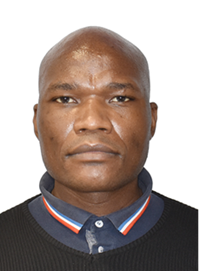
\includegraphics[width=1in,height=1.25in,clip,keepaspectratio]{Muwanei.png}}]{Sinyinda Muwanei} has worked as a lecturer and consultant in Zambia (Southern Africa) for more than eleven years. He has taught on BSc and MSc Information Technology programmes at various institutions of higher learning. Recently completed a PhD in Computer Science focusing on Information Retrieval Systems and Data Analytics.
\end{IEEEbiography}

\EOD
\end{document}
